%\documentclass[10pt,dvipsnames,slidestop,table]{beamer}
\documentclass[slidestop,compress,serif,10pt]{beamer}
\mode<presentation>
\usepackage[accumulated]{beamerseminar}
\usepackage{beamertexpower}
%\usepackage{beamerthemeshadow}
\usepackage{pdfpages}
\usepackage{animate}
\usepackage{varwidth, tikz, pgfgantt}
\usepackage[latin1]{inputenc}
\usepackage[T1]{fontenc}
\usepackage{graphicx}
\usepackage{pdfpages}
\usepackage{amsmath, amssymb, amsthm}
\usepackage{amsfonts}
\usepackage{xspace, array}
\usepackage{color, xcolor, bm}
\usepackage{fancybox}
\usepackage{caption}
\captionsetup[table]{position=top}
\setbeamertemplate{footline}[frame number]

\usepackage{hyperref}

\usepackage{natbib}
\bibpunct{(}{)}{;}{a}{}{,}
\setbeamertemplate{navigation symbols}{}
%\usecolortheme{seagull}
%\useoutertheme{infolines}
\usefonttheme{structuresmallcapsserif}
%\usefonttheme[onlymath]{serif}
%\usetheme{Singapore}
%\usecolortheme{beaver}
%\usetheme{Goettingen}
\usecolortheme{dolphin}


\title[]{Statistical modelling and challenges in environmental epidemiology}
\author[Marta Blangiardo]{Marta Blangiardo}
\institute[]{Imperial College London \\ MRC-PHE Centre for Environment and Heath\\
\scriptsize m.blangiardo@imperial.ac.uk\\
\vspace{12pt}
%\footnotesize \emph{Joint work with}: \\
%Monica Pirani, Lauren Kanapka, Gary Fuller, Nicky Best, Silvia Liverani, Richard Atkinson
}
\date[]{LSHTM, 17$^{th}$ October 2017}
%\logo{
\includegraphics[height=0.85cm, width=3.3cm]{LogoNew.jpg}\hspace{133pt}}
%\titlegraphic{
\includegraphics[height=0.85cm, width=3.3cm]{LogoNew.jpg}\hspace{133pt}}
\begin{document}
\begin{frame}
\maketitle
\begin{center}
%\footnotesize
%\emph{Joint work with}: \\
%\underline{Gary Fuller}, Nicky Best, Marta Blangiardo, Silvia Liverani, Richard Atkinson\\
\begin{figure}

\includegraphics[height=0.87cm, width=3.4cm]{LogoNew.jpg}
\end{figure}
\end{center}
\end{frame}

%%%%%%%%%%%%%%%%%%%%%%%%%%%%%%%%%%%%%%%%%%%%%%%%%%%%%%%%%%%%%%%%%
%%%%%%%%%%%%%%%%%%%%%%%%%%%%%%%%%%%%%%%%%%%%%%%%%%%%%%%%%%%%%%%%%
\section{Me}
\begin{frame}\frametitle{}
\begin{description}
\vfill\item[Who I am] 
Senior Lecturer in Biostatistics\\
Imperial College,
Department of Epidemiology and Biostatistics\\
MRC-PHE Centre for Environment and Health\\
\vspace{4pt}\begin{center}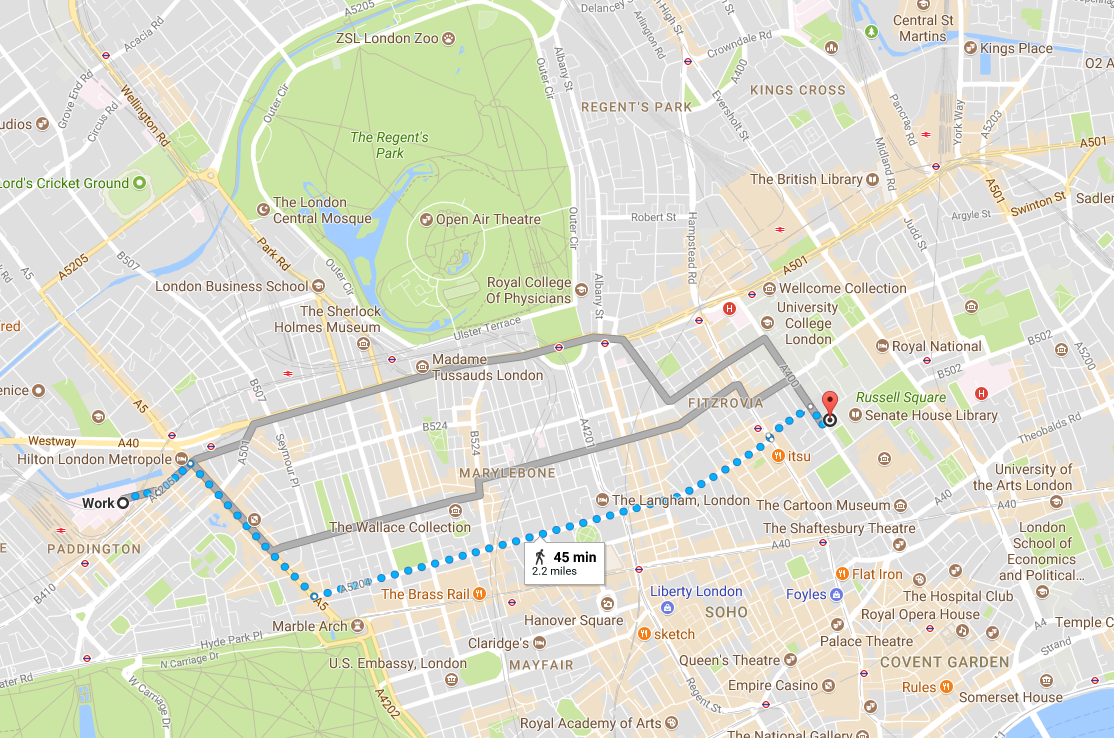
\includegraphics[width=6cm]{WorkMap.png}\end{center}
\vfill\item[What I do] Focus of my research is on the development of statistical methods to answer applied epidemiological questions.

%\item[My talk] I will present my work on \bf{spatial epidemiology}\\
%\begin{itemize}
%\item Two main areas: \\
%$\Rightarrow$ epidemiological surveillance\\
%$\Rightarrow$ risk assessment
%\end{itemize}
\end{description}  \end{frame}
%%%%%%%%%%%%%%%%%%%%%%%%%%%%%%%%%%%%%%%%%%%%%%%%%%%%%%%%%%%%%%%%%
\section{What is environmental epidemiology?}
%\begin{frame}
%\frametitle{Environmental epidemiology - definition}
%\begin{itemize}
%\vfill\item Epidemiology: The study of the distribution, causes and control of diseases in human population
%\vfill\item Disease risk depends on the classic epidemiological trio of person (in terms of genetics and behaviour), place and time -  spatial epidemiology focuses on the 2nd of these]
%\vfill\item Place is a surrogate for exposures present at that location, e.g. environmental exposures in water/air/soil, or the lifestyle characteristics of those living in particular areas
%\end{itemize}
%
%\begin{block}{}
%Describing and understanding spatial variation in disease risk and its link with environmental and other potential causes of disease.
%\end{block}
%\end{frame}

\begin{frame}\frametitle{Environmental Epidemiology}
\begin{itemize}
%\vfill\item Epidemiology: The study of the distribution, causes and control of diseases in human population.
%\vfill\item Disease risk depends on the classic epidemiological trio of person (in terms of genetics and behaviour), place and time.
\vfill\item Environmental epidemiology focuses on linking environmental hazards (exposures) to health outcomes. 
\begin{itemize}
\vfill\item Two main ingredients
\begin{itemize}
\item Environmental exposure\\
$\Rightarrow$ a continuous field over the study area.
\item Health outcomes\\
$\Rightarrow$ cohort / administrative data.
\end{itemize}
\pause\vspace{5pt}\item<1-> Study designs typically used:
\begin{itemize}
\vspace{5pt}\item<1-> Cohort studies - Focus on long-term effects (individual data);\vspace{3pt}
\vspace{5pt}\item<1-> Small area studies - Focus on long-term effects (aggregated data);\vspace{3pt}
\vspace{5pt}\item<1-> Time-series studies - Focus on short-term effects (aggregated data);\vspace{3pt}
\end{itemize}
\end{itemize}
\pause\begin{tikzpicture}[remember picture, overlay]
\draw[rounded corners=15pt,thick, red] (0.9,0.4) rectangle ++ (9.2,1.6);
\end{tikzpicture}

%\begin{block}{}
%Describing and understanding spatial variation in disease risk and its link with environmental causes of disease
%\end{block}
\end{itemize}
\alert{Spatial and temporal dependencies are keys.}
\end{frame}
%%%%%%%%%%%%%%%%%%%%%%%%%%%%%%%%%%%%%%%%%%%%%%%%%%%%%%%%%%%%%%%%%%%%%%%%%%%%%%%%%%%%%%%%%
%\begin{frame}\frametitle{Major player in Environmental Epidemiology}
%%\vspace{10pt} The two major players in environmental epidemiological studies are:
%\vfill\begin{itemize}
%\item Environmental exposure\\
%$\Rightarrow$ a continuous field over the study area;\\
%$\Rightarrow$ typically measured at points locations or modelled over a grid.
%\end{itemize}
%
%%\alert{Change of support issue}
%\vfill\begin{itemize}
%\item Health outcomes\\
%$\Rightarrow$ administrative registries / e-health data;\\
%$\Rightarrow$ typically aggregated over small administrative areas.
%\end{itemize}
%%\alert{Change of support and residual confounding issues}
%\vfill\centering\alert{Spatial and temporal dependencies are key.}
%\end{frame}
%%%%%%%%%%%%%%%%%%%%%%%%%%%%%%%%%%%%%%%%%%%%%%%%%%%%%%%%%%%%%%%%%


%\begin{frame}
%    \frametitle{Types of data}
%\begin{itemize}
%\vfill  \item \textbf{Point-referenced data}: the exact location of the case is known
%        \begin{itemize}
%\vfill        \item rarely available routinely, can be collected through case-control studies or specialized survey
%\vfill        \item if location itself is \emph{random}, e.g. measurements of where events occur\\
%         $\Rightarrow$ point process statistical framework
%\vfill        \item if locations are \emph{fixed} (monitoring stations, postcodes in an area)
%         and outcome is measured at each location (e.g. presence/absence of cases, pollution concentrations)\\
%         $\Rightarrow$ geostatistical framework
%        \end{itemize}
%\vfill  \item \textbf{Area data or count data}: locations are areal units with well defined geographical boundaries, usually administrative units
%        \begin{itemize}
%\vfill        \item outcome is number of cases aggregated over the area (and time)
%\vfill        \item most common type of data collected
%        \end{itemize}
%\end{itemize}
%\end{frame}

\begin{frame}
\frametitle{Why accounting for spatial and temporal dependencies is important}
	Spatial (temporal) patterns suggest that observations close to each other have more similar
	values than those far from each other.
%\vfill\item When are we interested in the spatial and temporal components?
\begin{itemize}
%\vfill	%\item Hypothesis generating perspective \\
\vspace{20pt}\item[] Are we explicitly interested in the spatial pattern of disease risk?\\
\item[] Do we want to evaluate temporal trends for each area?\\
\end{itemize}
\pause\begin{tikzpicture}[remember picture, overlay]
\draw[rounded corners=15pt,thick, red] (0.4,0) rectangle ++ (10.5,1.5)node[xshift=-5.5cm, yshift=0.1cm]{\fontsize{6}{7}\selectfont \sffamily Hypothesis generating};
\end{tikzpicture}

\begin{itemize}
\pause\vspace{20pt}\item[] Is the spatial clustering and/or temporal trend a nuisance quantity that we wish to take into account but are not explicitly interested in?\\ 
$\rightarrow$ Spatial regression / time series regression.\\
\end{itemize} 
\pause\begin{tikzpicture}[remember picture, overlay]
\draw[rounded corners=15pt,thick, red] (0.4,0.2) rectangle ++ (10.5,2.1)node[xshift=-5.5cm, yshift=0.1cm]{\fontsize{6}{7}\selectfont \sffamily Risk assessment};
\end{tikzpicture}
\end{frame}
%%%%%%%%%%%%%%%%%%%%%%%%%%%%%%%%%%%%%%%%%%%%%%%%%%%%%%%%%%%%%%%%%%%%%%%%%%%%%%%%%%%%%%%%
\begin{frame}\frametitle{Data/modelling/challenges in environmental epidemiology}
\begin{center}
\scalebox{.75}{\begin{tikzpicture}[remember picture, overlay]
\draw[rounded corners=15pt,thick] (-5,-5) rectangle ++ (3.1,5.2);
\draw[rounded corners=15pt,thick] (1.2,-5) rectangle ++ (3.1,5.2);
\draw[rounded corners=15pt,dashed] (-1.65,-4) rectangle ++ (2.6,4.0);
\draw(-3.5,-1.5) node[align=center,font=\sffamily\fontsize{7}{7}\selectfont](Exp){\\ Environmental exposure\\ e.g. air pollution\\ noise, pesticides};
\node[below=0.1 of Exp, align=center,font=\sffamily\fontsize{7}{7}\selectfont](Mes){Measurements};
\node[below=0.1 of Mes, align=center,font=\sffamily\fontsize{7}{7}\selectfont](Mod){Modelled};
\node[above=0.5 of Exp, text=blue,align=center,font=\sffamily\fontsize{7}{7}\selectfont](Methods1){Space-time regression};
\node[below=0.5 of Mod, text=red,align=center,font=\sffamily\fontsize{7}{7}\selectfont](Chall1){Misalignment;\\ Measurement error;\\ Correlated data;\\ Computational (big data)};
\node[right=4 of Exp, align=center,font=\sffamily\fontsize{7}{7}\selectfont](Health){Health data\\ (EHR)\\};
\node[below=0.1 of Health, align=center,font=\sffamily\fontsize{7}{7}\selectfont](HES){Hospital Admissions};
\node[below=0.5 of HES, align=center,font=\sffamily\fontsize{7}{7}\selectfont](Mort){Mortality Registry};
\node[above=0.5 of Health, text=blue,align=center,font=\sffamily\fontsize{7}{7}\selectfont](Methods2){Clustering;\\ Disease surveillance};
\node[below=0.5 of Mort, text=red,align=center,font=\sffamily\fontsize{7}{7}\selectfont](Chall2){Correlated conditions;\\ Space-time modelling};
\draw [->,>=latex,shorten >=5pt,shorten <=5pt,auto,node distance=5pt, thick] (Exp.east) to (Health.west);
\node[below right = 0.4 of Exp, align=center,font=\sffamily\fontsize{7}{7}\selectfont, text=red](Chall3){Correlation;\\ Residual confounding;\\ Dose-response};
\node[above=1.1 of Chall3, text=blue,align=center,font=\sffamily\fontsize{7}{7}\selectfont](RA){Risk assessment};

\node[below=4.2 of RA, align=center,font=\sffamily\fontsize{7}{7}\selectfont, text=red](Overarching){Data integration, Uncertainty propagation \& feedback;  Missing data};

\end{tikzpicture}}
\end{center}

\vspace{4cm}
In this talk\\
\begin{itemize}
\item Two main areas: \\
$\Rightarrow$ disease surveillance (space-time modelling);\\
$\Rightarrow$ risk assessment (residual confounding and correlated exposures).
\end{itemize}
%\begin{center}\alert{Overarching theme: spatial epidemiology}\end{center}
\end{frame}

%%%%%%%%%%%%%%%%%%%%%%%%%%%%%%%%%%%%%%%%%%%%%%%%%%%%%%%%%%%%%%%%%
\section{Modelling framework for small area data}
%\begin{frame}
%\frametitle{Commonly used methods for surveillance}
%\begin{description}
%\vfill\item[Statistical tests]: test a subset of data defined by spatio-temporal constraints against an expected rate of disease occurrence over the study area.
%\begin{enumerate}
%\vfill\item Scan statistics
%\vfill\item CUSUM
%\end{enumerate}
%\vfill\item[Model based approaches]: used to adjust for the expected number of cases; can include confounders; flexible space and time trends. 
%\begin{enumerate}
%\vfill\item Hierarchical framework (Bayesian or frequentist)
%\end{enumerate}
%\end{description}
%\end{frame}
%%%%%%%%%%%%%%%%%%%%%%%%%%%%%%%%%%%%%%%%%%%%%%%%%%%%%%%%%
%\subsection*{Scan statistic}
%\begin{frame}\frametitle{Scan Statistic}
%\begin{itemize}
%\vfill\item Mostly used in outbreak detection
%\vfill\item Spatial search: Circular windows of varying radii scan a map of disease and test if the number of cases is larger than the expected ones
%\vfill\item Can be extended to spatio-temporal search using cylinders instead of circles (height of cylinder corresponds to time periods of varying lengths)
%\vfill\item Monte Carlo simulation is used to assess the presence of a cluster
%\vfill\item Software: SatScan - R package \texttt{rsatscan}
%\end{itemize}
%\end{frame}
%%%%%%%%%%%%%%%%%%%%%%%%%%%%%%%%%%%%%%%%%%%%%%%%%%%%%%%%%
%\subsection*{CUSUM}
%\begin{frame}\frametitle{CUSUM}
%\begin{itemize}
%\vfill\item Running sum of deviations of observed cases from expected values
%\vfill\item Once it reaches a threshold it triggers an alarm
%\vfill\item For space-time applications individual cumulative sums for each area under surveillance are monitored and can be adjusted for spatial relationship
%\vfill\item Software:R package \texttt{qcc}
%\end{itemize}
%\end{frame}
%%%%%%%%%%%%%%%%%%%%%%%%%%%%%%%%%%%%%%%%%%%%%%%%%%%%%%%%%
\begin{frame}\frametitle{Small area modelling framework}
When dealing with aggregated data at the small area level
\begin{itemize}
\item The easiest model consists in specifying the observed counts of events for area $i$ ($i=1,\ldots,N$) as
\begin{equation*} O_i \sim \hbox{Poisson}(\lambda_i E_i) \end{equation*}
 
 \begin{itemize}
 \item SMR$_i= \frac{O_i}{E_i}$ is the MLE for $\lambda_i$
\item SMR$_i$ very imprecise for rare diseases and/or areas with small populations, $\lambda_i$ estimated variance is $\frac{O_i}{E_i^2}$\\
$\Rightarrow$ Highlights extreme risk estimates based on small numbers.
    \end{itemize}
\vspace{0.2cm}
\pause\item SMR in each area is estimated independently\\
$\rightarrow$ makes no use of risk estimates in other areas of the map, even though these are likely to be similar.
\vspace{0.2cm}
\item Ignores possible spatial correlation between disease risk in nearby areas 
\end{itemize}

\pause\centering\color{red}{Bayesian `smoothing' estimators in a hierarchical formulation.}

\end{frame}
%%%%%%%%%%%%%%%%%%%%%%%%%%%%%%%%%%%%%%%%%%%%%%%%%%%%%%

\begin{frame}
    \frametitle{Hierarchical modelling for small area data}
\begin{block}{Poisson-logNormal model}
\vspace{-0.5cm}
\begin{eqnarray*}
O_i & \sim & \hbox{Poisson}(\lambda_i E_i) \\
\log \lambda_i & = & \alpha + v_i\\
v_i & \sim  & \hbox{Normal}(0, \sigma_v^2)
\end{eqnarray*}

%{\small
%Priors (vague, non informative):
%\vspace{-0.2cm}
%\begin{itemize}
%  \item between-area sd: $\sigma_v \sim \text{Truncated Normal}(0,100)_{[0,Inf)}$
%  \vspace{-0.2cm}
%  \item mean log relative risk: $\alpha \sim flat()$
%\end{itemize}}
\end{block}
where
\begin{itemize}
  \item $O_i$, $E_i$: observed and expected nb of cases in area $i$
  \item $\lambda_i=\exp (\alpha +  v_i)$: RR in area $i$ compared with expected risk based on age and sex of population
  \item Parameters $v_i$: {\bf area-specific random effects}
  \item residual RR = $\exp (v_i)$
% \lambda as relative risk (number of cases in the area compared to the expected - accounting for all the risk factors in the area compared with the normal age and sex in the population
\end{itemize}
\end{frame}
%%%%%%%%%%%%%%%%%%%%%%%%%%%%%%%%%%%%%%%%%%%%%%%%%%%%%%%%
\begin{frame}
    \frametitle{Lung cancer incidence in males, 1985-2009, England and Wales (I)}
    \begin{center}
    RR estimates using 2 methods
        \scalebox{0.6}{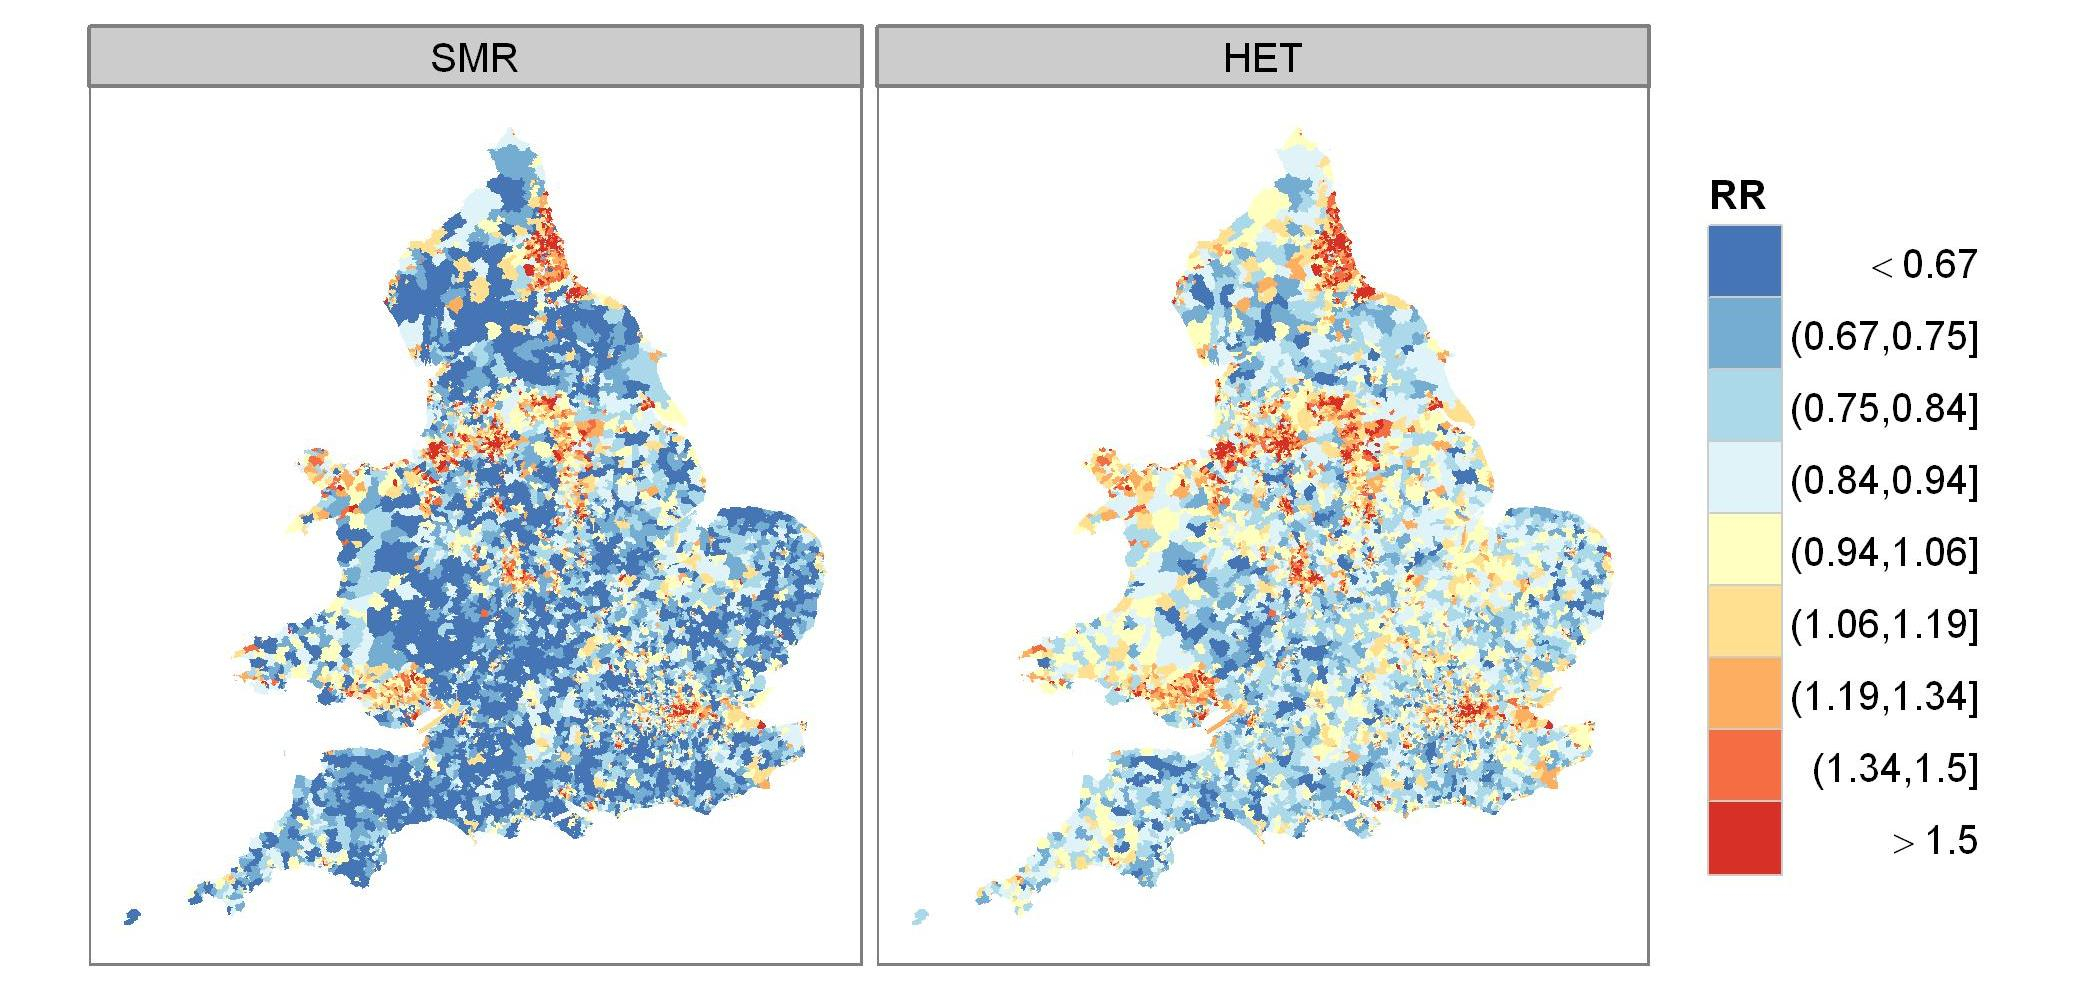
\includegraphics{Lungmales_SMRHETmap.jpg}}\\
        SMRs and smoothed RRs
    \end{center}
\end{frame}

%%%%%%%%%%%%%%%%%%%%%%%%%%%%%%%%%%%%%%%%%%%%%%%%%%%%%%%%
\begin{frame}\frametitle{Local spatial dependency}
To account for local dependency it is possible to add a spatial structure in the model:
\begin{block}{Convolution model}
\vspace{-0.5cm}
\begin{eqnarray*}
O_i & \sim & \hbox{Poisson}(\lambda_i E_i) \\
\log \lambda_i & = & \alpha + v_i + u_i\\
v_i & \sim  & \hbox{Normal}(0, \sigma_v^2)\\
u_i \mid u_{-i} & \sim & \hbox{Normal}\left(\frac{\sum_{k=1}^n w_{ik} u_k}{\sum_{k=1}^n w_{ik}}, \frac{\sigma^2_u}{\sum_{k=1}^n w_{ik}}\right)\end{eqnarray*}
\end{block}
\begin{itemize}
  \item $u_i$ follows a conditional autoregressive specification (CAR); it assumes that only neighbouring areas contribute to the distribution of area $i$ ($w_{ik}=1$).
  \item The combination of $v_i$ and $u_i$ guarantees local and global smoothing (BYM model).
\end{itemize}

%\fontsize{7}{7}\selectfont{Besag, J., et al. (1991). ``Bayesian image restoration, with two applications in spatial statistics''. \textbf{Annals of the Institute of Statistical Mathematics}, 43, 1-59.}
\end{frame}
%%%%%%%%%%%%%%%%%%%%%%%%%%%%%%%%%%%%%%%%%%%%%%%%%%%%%%%%

\begin{frame}\frametitle{Residual RR of lung cancer incidence in males, 1985-2009, England and Wales II}
\begin{center}\begin{tikzpicture}[remember picture, overlay]
  \node (img1) at (-2.8,-3.2) {{\visible<1->{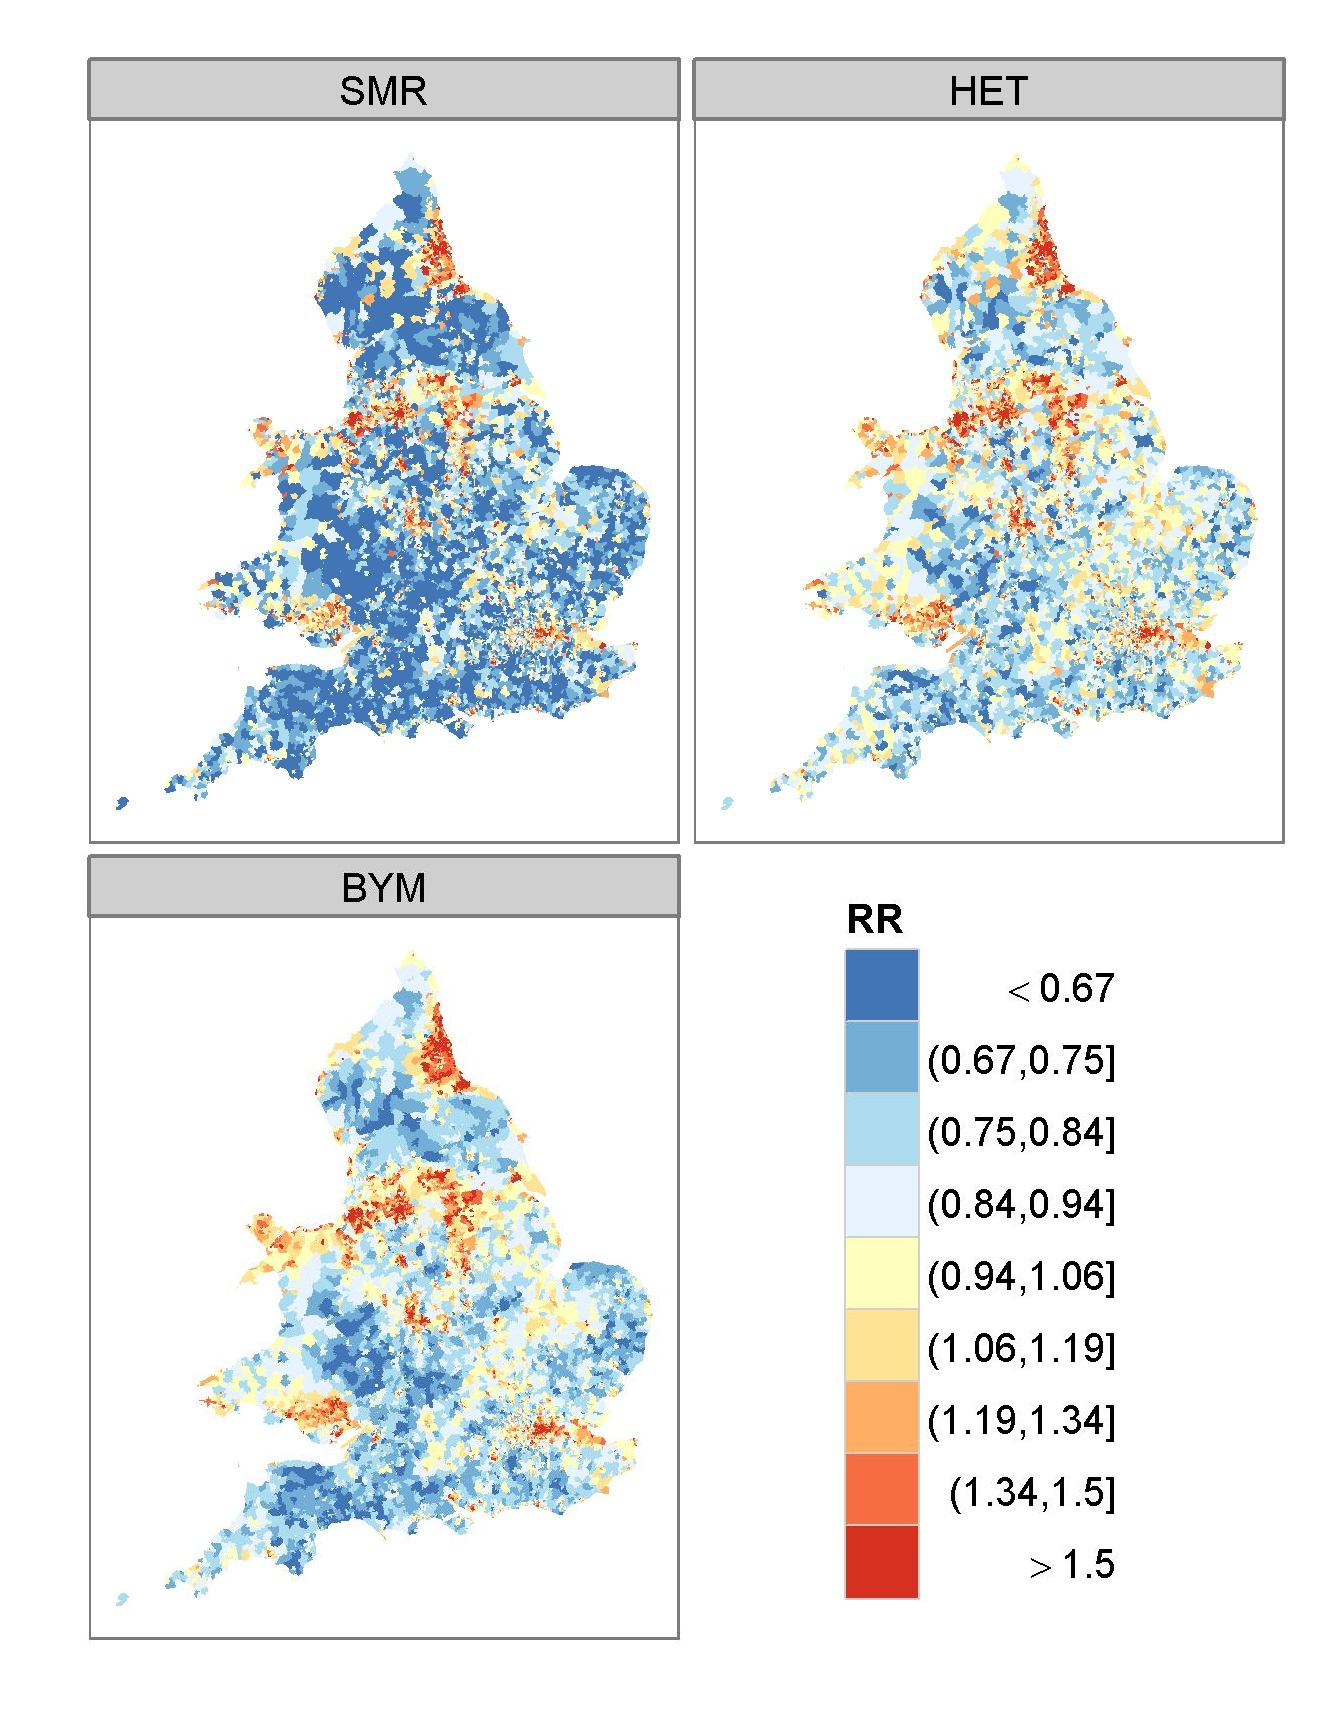
\includegraphics[scale=.5]{Lungmales_3maps.jpg}}}};
  \node[right=1cm of img1,text width=5cm](text){\textbf{SMR}: non smoothed RR\\ \vspace{10pt}\textbf{HET}: non spatially smoothed residual RR $\exp(v)$\\ \vspace{10pt}\textbf{BYM}: spatially and non spatially smoothed residual RR $\exp(v+u)$};
\end{tikzpicture}
\end{center}
\end{frame}

%%%%%%%%%%%%%%%%%%%%%%%%%%%%%%%%%%%%%%%%%%%%%%%%%%%%%%%%%%%%%%%%%%%%%%%%%%%%%%%%%%%%%%%%%%
\frame{\frametitle{From spatial to spatio-temporal modelling}
\begin{itemize}
\vfill \item The hierarchical structure can be extended to incorporate time into a space-time model.
\vfill \item The stability (or not) of the
spatial pattern can aid interpretation.
\vfill \item The specific
space-time components of the model can potentially pinpoint
unusual / emerging hazards.
\end{itemize}

\begin{block}{Spatio-temporal hierarchical model}
\vspace{-0.5cm}
\begin{eqnarray*}
O_{it} & \sim & \hbox{Poisson}(\lambda_{it} E_{it}) \\
\log \lambda_{it} & = & \alpha + v_i + u_i + \phi_t + \psi_{it}\\
\end{eqnarray*}

{\small
Temporal trend and space-time interaction:
\vspace{-0.2cm}
\begin{itemize}
  \item Temporal trends: $\phi_t \sim \text{Normal}(\phi_{t-1}, \sigma^2_{\phi})$
  \vspace{-0.2cm}
  \item Space-time interaction: $\psi_{it} \sim \text{Normal}(0,\sigma^2_{\psi})$
\end{itemize}}
\end{block}

}

%\frame{\frametitle{Schematic representation I}
%\begin{center}
%\scalebox{0.45}
%{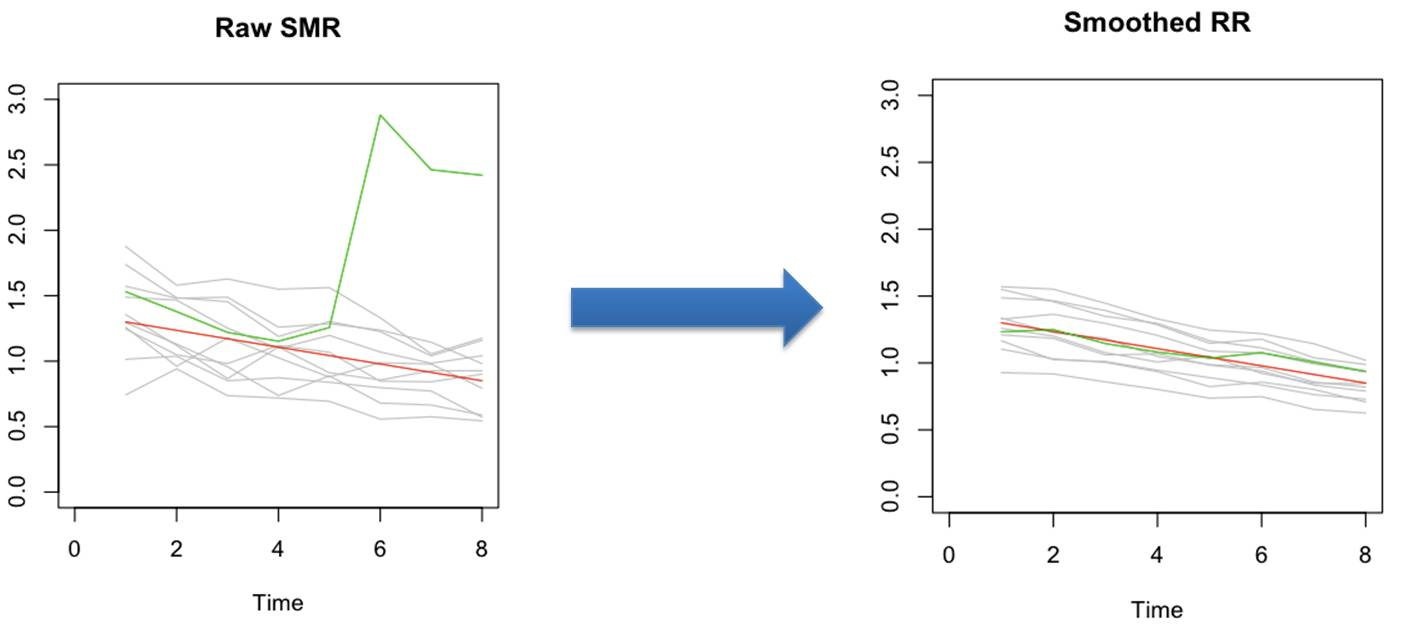
\includegraphics{representation_ST1.jpg} }
%\end{center}
%}

\frame{\frametitle{Schematic representation}
\begin{center}
\scalebox{0.45}
{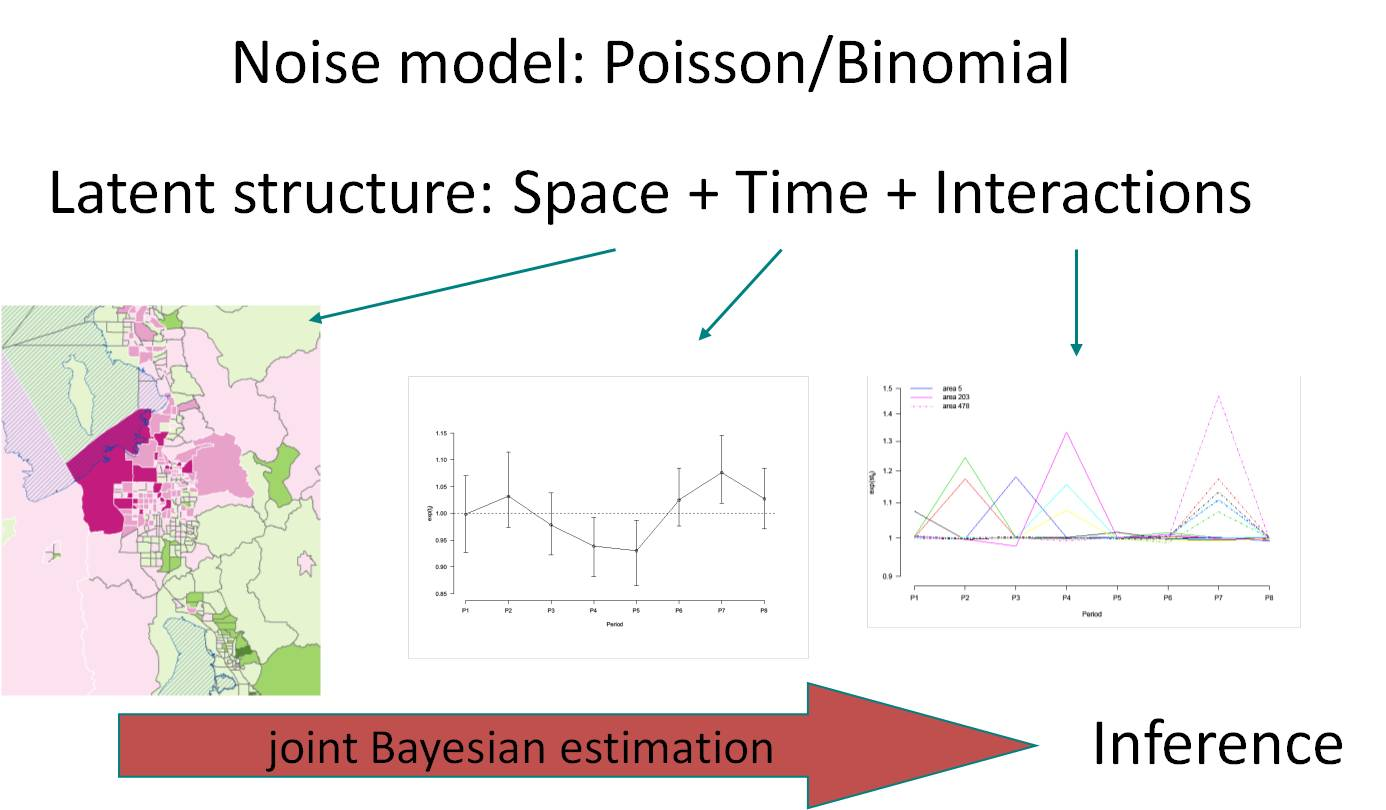
\includegraphics{representation_ST.jpg} }
\end{center}
}
%%%%%%%%%%%%%%%%%%%%%%%%%%%%%%%%%%%%%%%%%%%%%%%%%%%%%%%%
%\begin{frame}{Disease surveillance for COPD admissions}

% \begin{block}{}
%\centering
%\begin{itemize}
%\item To specify a spatio-temporal model to investigate for disease surveillance.\\
%\item Several applications: COPD mortality, Cancer Incidence, Traffic Accidents injuries
%\end{itemize}
%\end{block}
%  \vskip0pt plus.5fill
%
%\pause 
%Extend the spatio-temporal hierarchical framework to a mixture model with two components
%
%    \begin{itemize}
%    \vfill\item accounts for spatial  and temporal correlation
%\vfill\item
%able to detect areas with trend different from the national one (unusual)
%   \end{itemize}
%
%\end{frame}

%%%%%%%%%%%%%%%%%%%%%%%%%%%%%%%%%%%%%%%%%%%%%%%%%%%%%%%%
\section{Disease surveillance}\begin{frame}
\begin{center}
\vfill\fontsize{20}{20}\selectfont{Disease Surveillance}\end{center}
\end{frame}

\begin{frame}
\frametitle{Disease surveillance: why}
 \begin{block}{}
Surveillance is a key practice within the NHS to ensure that the right information is available at the right time to inform public health decisions and interventions. 

\vspace{5pt} It is the ongoing systematic data collection, analysis, interpretation and dissemination of information in order for action to be taken. 
\end{block}

\vspace{20pt} Appropriate for a wide range of problems:
\begin{itemize}
\item to investigate the epidemiology of a public health issue;
\item to assess an impact of an intervention/policy;
\item to provide early warning detection.
\end{itemize}
\end{frame}
%%%%%%%%%%%%%%%%%%%%%%%%%%%%%%%%%%%%%%%%%%%%%%%%%%%%%%%%
\begin{frame}
\frametitle{Disease surveillance: examples}
Several areas where surveillance models have been used
\vfill\begin{enumerate}
\vfill\item medical malpractice and failures to deliver appropriate standards of health care (ex. \citet{Marshall:2004}); 
\vfill\item outbreaks of communicable diseases (ex. \citet{WHOsurv});
%\vfill\item against the threat of bio-terrorism;
\vfill\item discover unusual trends in non-communicable diseases (ex. \citet{kxs005}).
\end{enumerate}

\vspace{20pt} \begin{block}{}
In these contexts the data are characterised by a spatial and temporal dimension and therefore appropriate surveillance methods that are able to capture \alert{spatial and temporal patterns} need to be employed. 
\end{block}
\end{frame}
%%%%%%%%%%%%%%%%%%%%%%%%%%%%%%%%%%%%%%%%%%%%%%%%%%%%%%%%\begin{frame}{Background: COPD}
\begin{frame}\frametitle{Disease surveillance for COPD}
 \begin{block}{}
COPD\footnote{Chronic Obstructive Pulmonary Disease}  is one of the most common chronic respiratory diseases (CRDs), that affect the airways and other structures of the lung (WHO, 2012).
\end{block}

\begin{itemize}
\vfill\item 64 million people currently suffering from the disease;
\vfill\item Responsible for 6\% of deaths worldwide; projection to become the 3rd leading cause of death by 2030 (WHO, 2014);
\vfill\item 5th cause of death in UK.
\end{itemize}

\end{frame}
%%%%%%%%%%%%%%%%%%%%%%%%%%%%%%%%
%\begin{frame}\frametitle{COPD statistics: diagnosis}
%
%\begin{center}
%\begin{tikzpicture}
%  \node (img1) {{\visible<1->{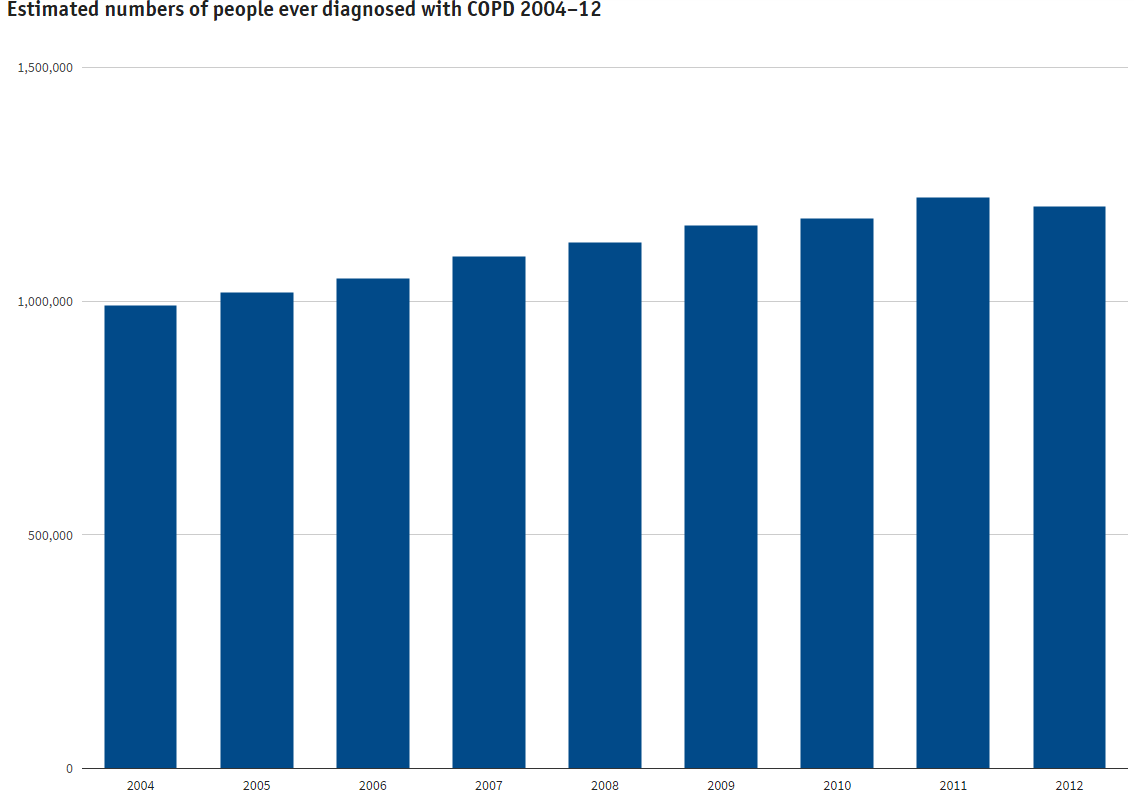
\includegraphics[height=4cm]{COPDdiagnosis.png}}}};
%  \pause
%  \node (img2) at (img1.south east) {{\visible<2->{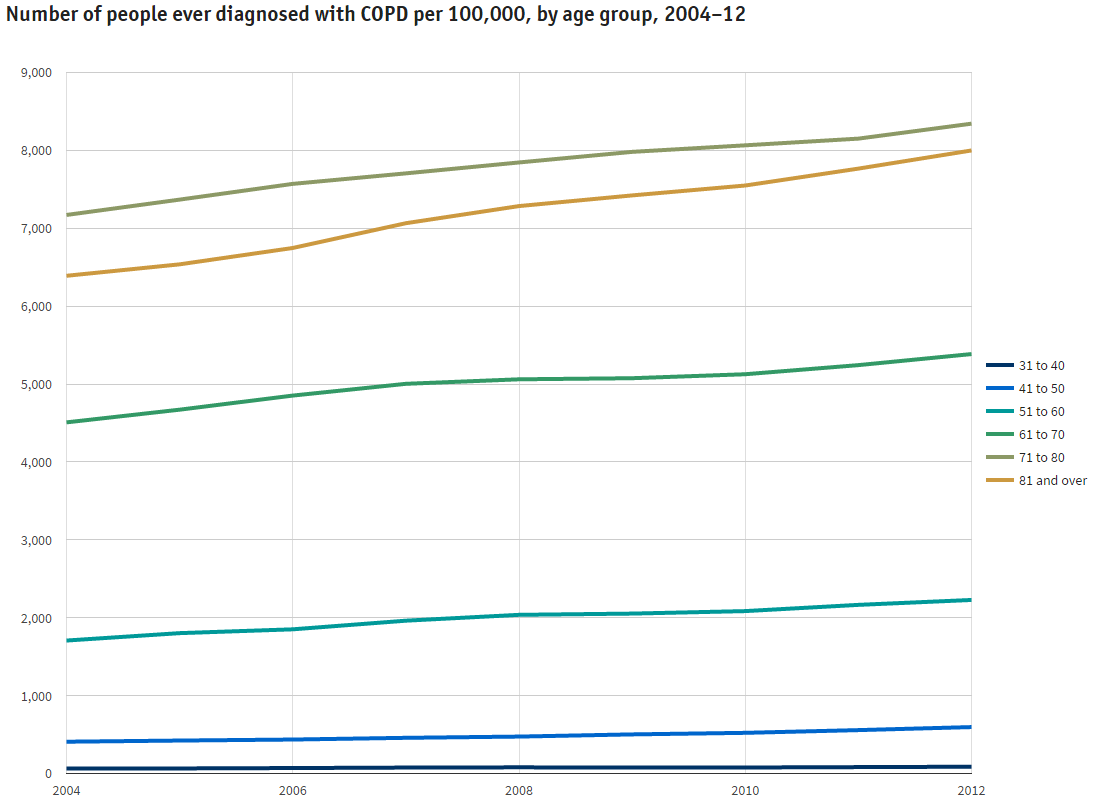
\includegraphics[height=4cm]{COPDage.png}}}};
%  \pause
%  \node (img3) at (img2.south west) [yshift=1cm] {{\visible<3->{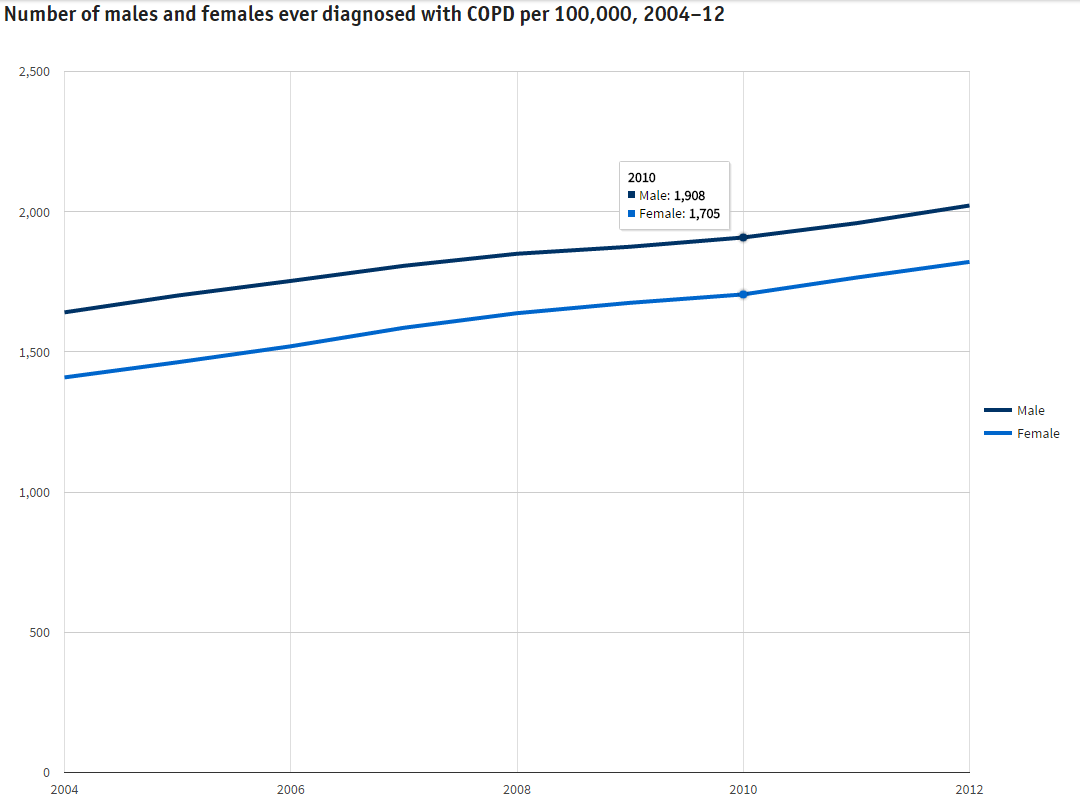
\includegraphics[height=4cm]{COPDsex.png}}}};
%\end{tikzpicture}
%\end{center}
%
%\begin{footnotesize}
%Source: British Lung Foundation
%\end{footnotesize}
%\end{frame}
%
%%%%%%%%%%%%%%%%%%%%%%%%%%%%%%%%
%\begin{frame}
%\frametitle{COPD statistics: hospital admissions}
%\begin{columns}
%\begin{column}{0.5\linewidth}
%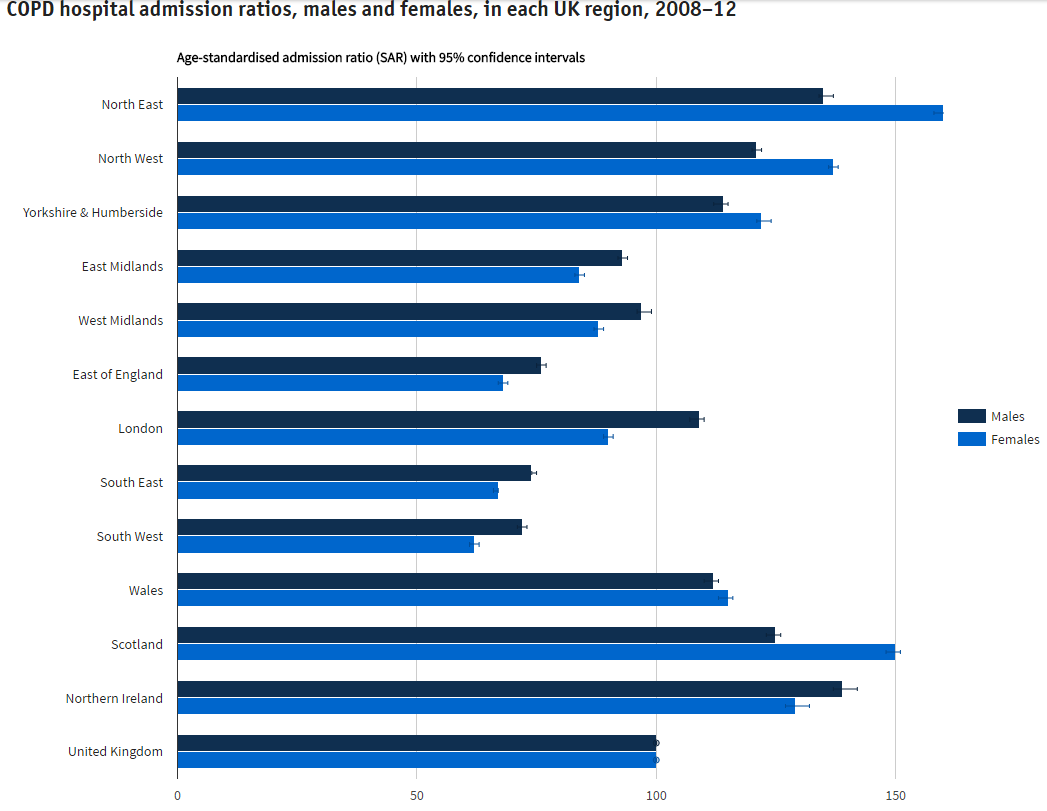
\includegraphics[height=5cm]{COPDhes.png}
%\end{column}
%
%\begin{column}{0.4\linewidth}
%\begin{itemize}
%\item Geographical variation
%\item North-South trend
%\item Very large areas  - need to go to higher spatial resolution and incorporate time
%\end{itemize}
%\end{column}
%\end{columns}
%\end{frame}

%%%%%%%%%%%%%%%%%%%%%%%%%%%%%%%
\begin{frame}{Maps of Crude Rates}

 \begin{block}{}
\small{Spatial resolution: 211 Clinical Commissioning Groups (CCGs)\\
Temporal resolution: monthly data, April 2010 - March 2011.\\
}
\end{block}
 % \vskip0pt plus.5fill
\centering
\begin{figure}\caption{Hospital Episode Statistics (HES) SMRs}
\animategraphics[autoplay,loop, width=4.8cm]{1}{SMR}{1}{12}
\end{figure}
\end{frame}
%%%%%%%%%%%%%%%%%%%%%%%%%%%%%%%%%%%%%%%%%%%%%%%%%%%%%%%%%%%%%%%%


%%%%%%%%%%%%%%%%%%%%%%%%%%%
\begin{frame}{Spatio-temporal mixture model}
\begin{itemize}
\item Extend the spatio-temporal hierarchical framework to a mixture model with two components
    \begin{itemize}
    \vfill\item accounts for spatial  and temporal correlation;
\vfill\item able to detect areas with trend different from the national one (unusual).
   \end{itemize}
\end{itemize}

 \center{$O_{it} \sim \mbox{Poisson}(\lambda_{it}\; E_{it})$}
  \vskip0pt plus.5fill
\small{areas  $i=1, \dots, 211$; time points $t=1, \dots, 12$}.
\medskip
\begin{align*}
\begin{split}
 \mbox{log} (\lambda_{it}) = p_{it} \;  \mbox{log}\big(\,\lambda_{it}^{\mbox{C}}\,\big)  + (1-p_{it}) \; \mbox{log}\big(\, \lambda_{it}^{\mbox{AS}}\, \big)  
\end{split}
\end{align*}
\centering



\begin{tikzpicture}
\draw[blue, thick, ->] (0.8,0) -- (1.5, -1);
\draw[blue, thick, ->] (-0.8,0) -- (-1.5,-1);
\end{tikzpicture}


\begin{columns}
\begin{column}[T]{0.37\textwidth}
\centering
\textcolor{blue}{Common Trend}
\begin{itemize}
\item[$\bullet$] overall intercept
\item[$\bullet$]  spatial component
\item[$\bullet$]  temporal component
\end{itemize}
%\[  \mbox{log}\big(\,\mu_{it}^{\mbox{C}}\,\big) =\quad  \alpha_0 + h_i + \gamma_t\]
%\[  \alpha_0 \sim  \quad \mbox{U}(-\infty, +\infty)\]
%\[ h_i \sim \mbox{N}(v_i,\sigma^2_h) \; \; and \;  \; v_i \sim \mbox{CAR}(\mbox{W}, \sigma^2_v)\]
%\[ \gamma_{t} \sim  \quad \mbox{CAR}(\mbox{Q}, \sigma^2_\gamma) \]
\end{column}
\begin{column}[T]{0.4\textwidth}
\textcolor{blue}{Area-Specific Trend}
\centering
\begin{itemize}
\centering
\item[$\bullet$]  area-specific intercept
\item[$\bullet$] area-specific temporal component
\end{itemize}
%\[ \mbox{log}\big(\, \mu_{it}^{\mbox{AS}}\, \big)=  \quad u_i + k_{it}\]
%\[ u_i \sim \quad \mbox{N}(0,1000) \]
%\[k_{i, t} \sim  \quad \mbox{CAR}(\mbox{Q}, \sigma^2_{i,k}) \]
%\[\mbox{log}(\sigma^2_{i,k}) \sim  \quad \mbox{N}(\alpha, \beta^2) \]
\end{column}
\end{columns}


\end{frame}

%%%%%%%%%%%%%%%%%%%%%%%%%
\begin{frame}
\frametitle{Modelling the probability for the two components}
\begin{itemize}
\item Each area is characterised by a (vector of) probability $\bm p_{i}=\left( p_{i1}, \ldots, p_{iT} \right)$ of being assigned to the common trend component
\item $p_{it}$ can be modelled as a combination of several effect:
\begin{itemize}
\item local and global dependency in space (clusters or isolated areas)\\
\begin{center}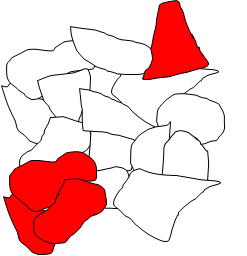
\includegraphics[scale=0.3]{Cluster.png}\end{center}
\item local and global dependency in time (similar trend or isolated time points)\\
\begin{center}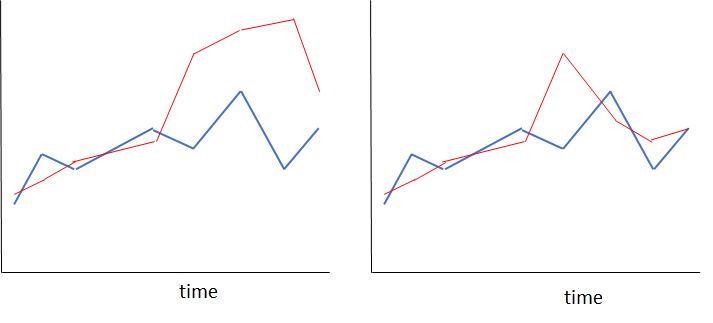
\includegraphics[scale=0.3]{TimeCluster.png}\end{center}
\end{itemize}
\end{itemize}
\end{frame}
%%%%%%%%%%%%%%%%%%%%%%%%%%
%\begin{frame}
%\frametitle{Implementation}
%\begin{itemize}
%\vfill\item Bayesian formulation - priors on all the parameters
%\vfill\item Inference is performed through Markov Chain Monte Carlo simulative approach
%\vfill\item The model is currently implemented in OpenBUGS via R\end{itemize}
%\end{frame}

%%%%%%%%%%%%%%%%%%%%%%%%%
\begin{frame}{Results: Spatial \& Temporal Patterns}

%\begin{figure}[h]
\begin{tabular}{m{5cm}m{5cm}}
\footnotesize{Spatial Posterior Mean} & \hspace{30pt}\footnotesize{Unusual Areas}\\
\end{tabular}
\begin{columns}
\begin{column}{0.5\textwidth}               
%\begin{subfigure}[b]{0.45\textwidth} 
%               \caption{\footnotesize{Spatial Posterior Mean}}
%\footnotesize{Spatial Posterior Mean}\\
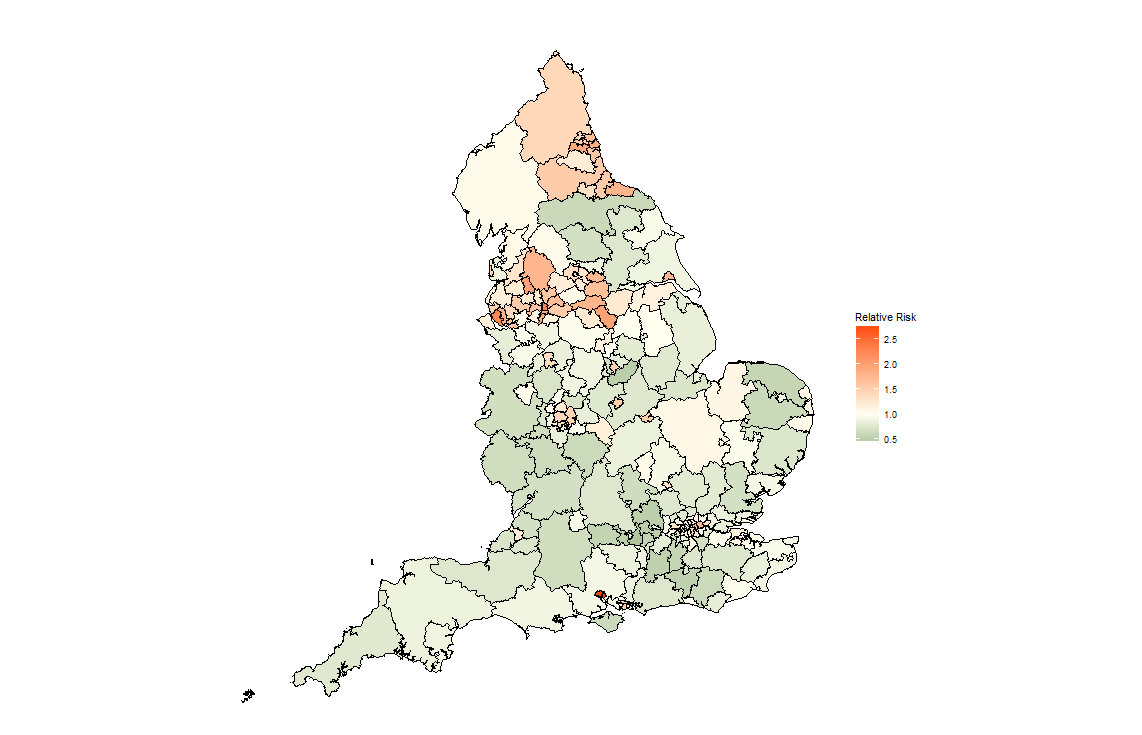
\includegraphics[width=\textwidth]{RRmap}
\end{column}

                 %\end{subfigure}
%            \begin{subfigure}[t]{0.55\textwidth}
%            \caption{\footnotesize{Unusual areas}}
\begin{column}{0.5\textwidth}               
%\footnotesize{Unusual Areas}\\
                 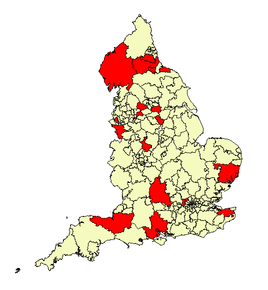
\includegraphics[width=0.6\textwidth]{outbreaks_map}
\end{column}
\end{columns}
%        \end{subfigure}
%\end{figure}
\begin{itemize}
\vfill\item Higher risk in the north of England across the time period
\vfill\item Unusual areas: Mostly isolated but some clustered in the North of England
\end{itemize}

\fontsize{7}{7}\selectfont{
Boulieri A, Hansell A, Blangiardo M, ``Investigating trends in asthma and COPD through multiple data sources: A small area study'', \textbf{Spatial and SpatioTemporal Epidemiology}, 2016, 19: 28-36.
}

\begin{center}
\pause\begin{tikzpicture}[overlay]
  \node (img1) at (-0.1,3.3) {{\visible<1->{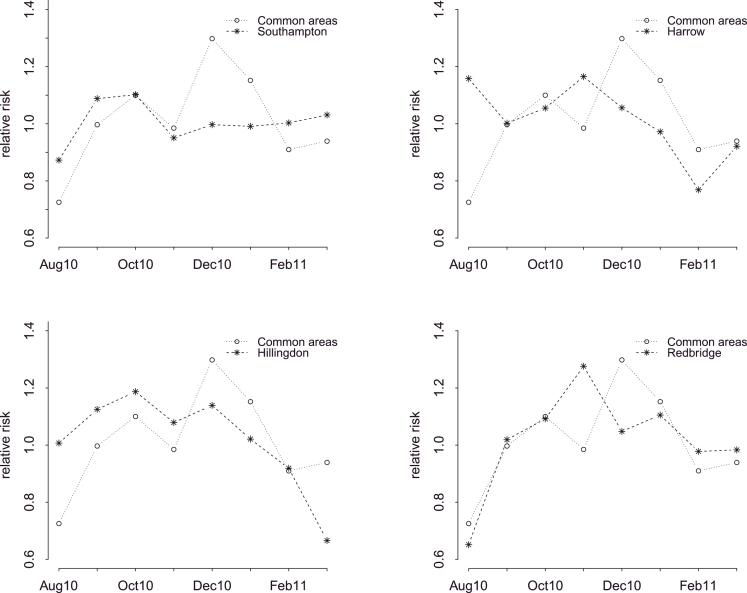
\includegraphics[height=8.3cm]{gr4}}}};
%  \pause
%  \node (img2) at (0,-1.7) {{\visible<2-2>{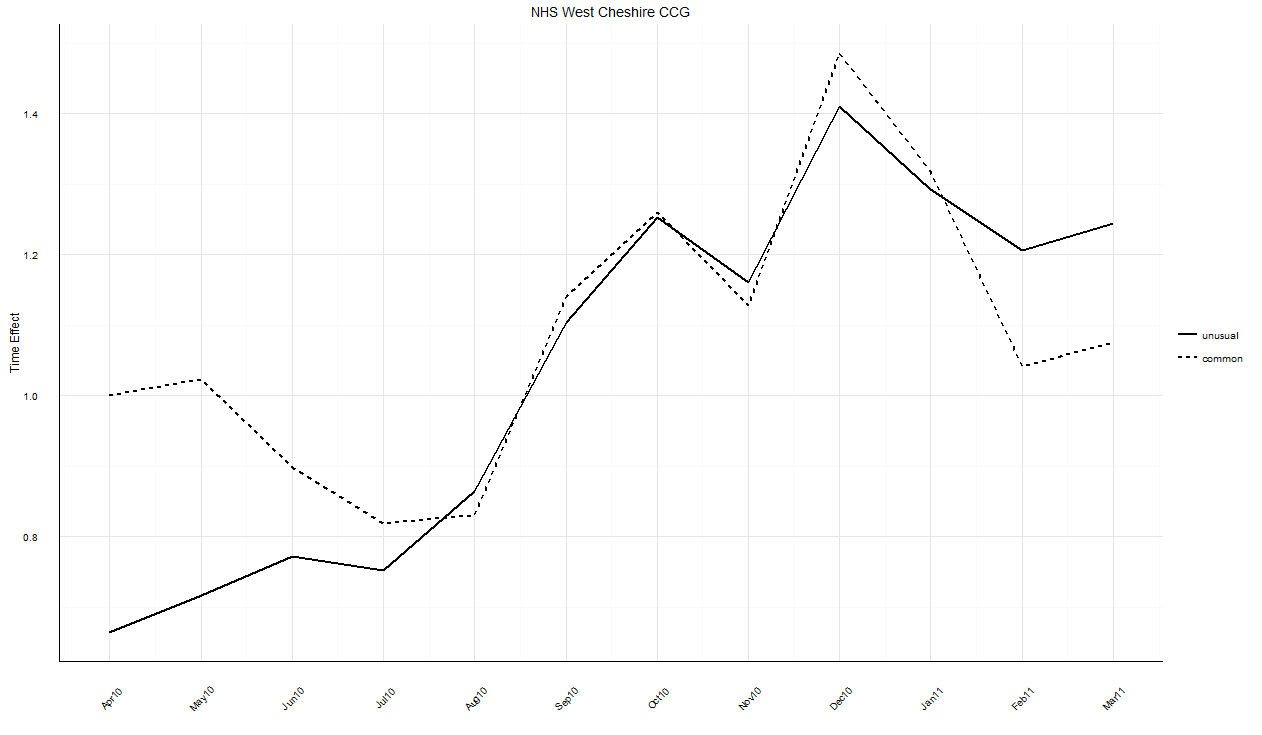
\includegraphics[height=5cm]{Cheshire.png}}}};
%  \pause
% \node (img3) at (0,-2.7){{\visible<3-3>{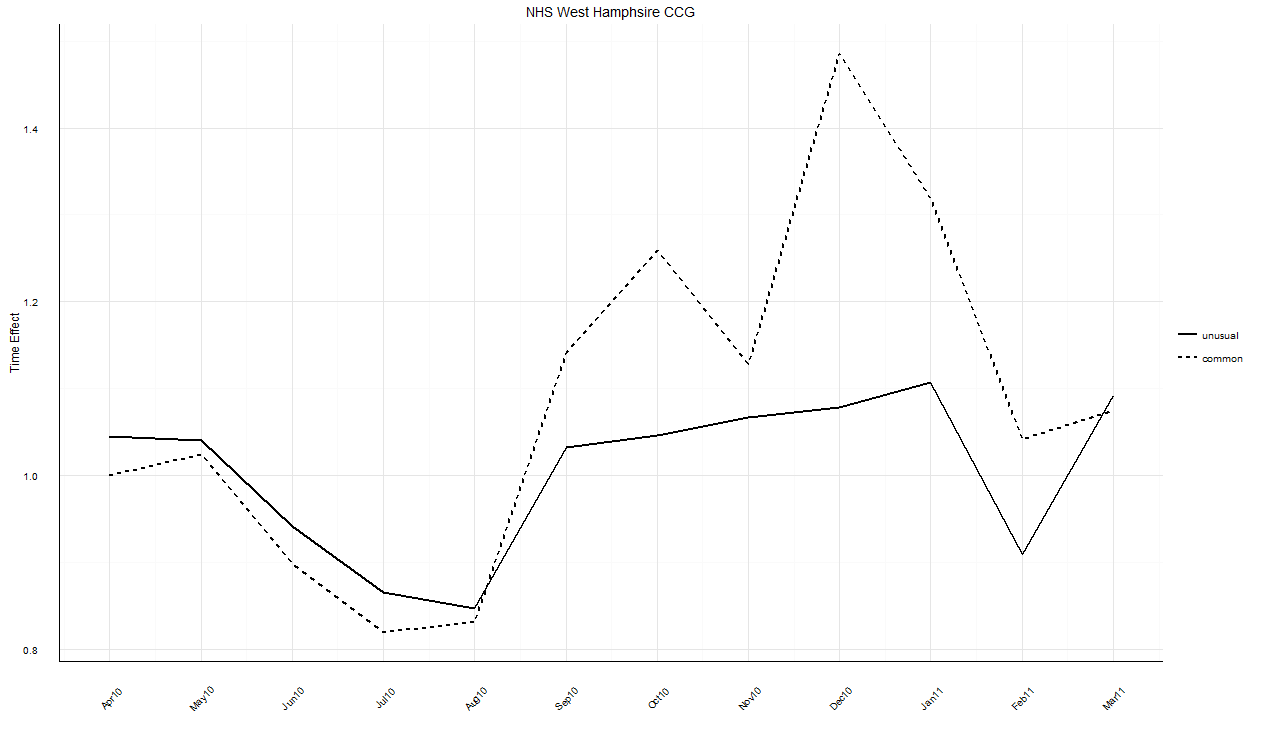
\includegraphics[height=5cm]{Hamphsire.png}}}};
% \pause
%  \node (img4) at (0,-3.7) {{\visible<4-4>{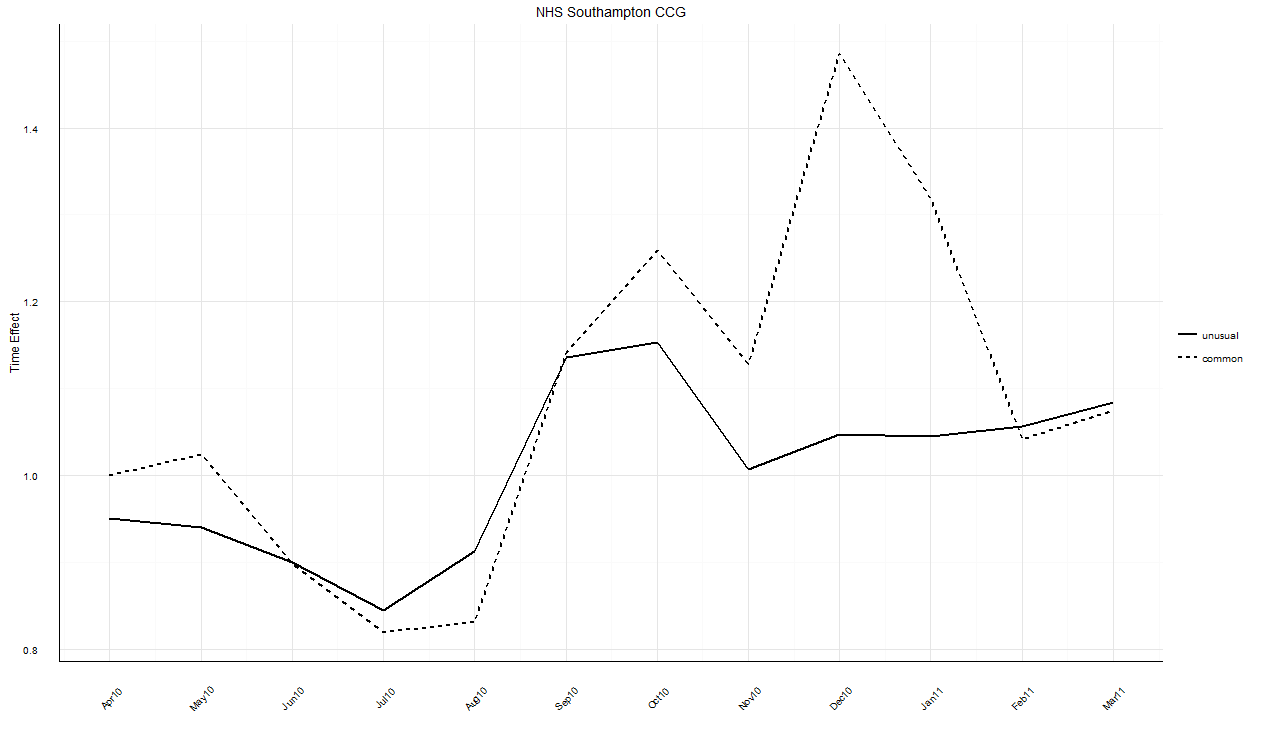
\includegraphics[height=5cm]{Southampton.png}}}};
% \pause
%  \node (img5) at (0,-4.7) {{\visible<5-5>{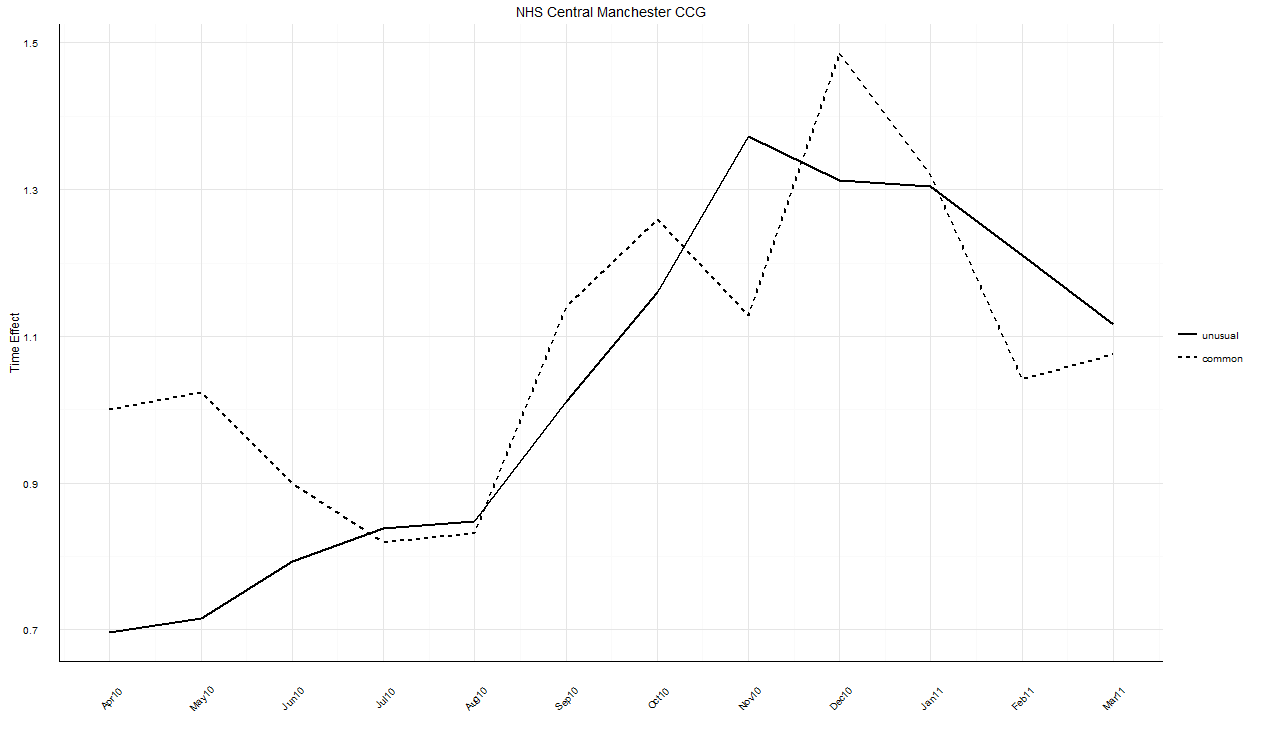
\includegraphics[height=5cm]{Manchester.png}}}};  
\end{tikzpicture}
\end{center}

%\end{frame}

%\begin{frame}
%\begin{center}
%\begin{tikzpicture}[overlay]
%  \node (img1) at (0,-2.7) {{\visible<1->{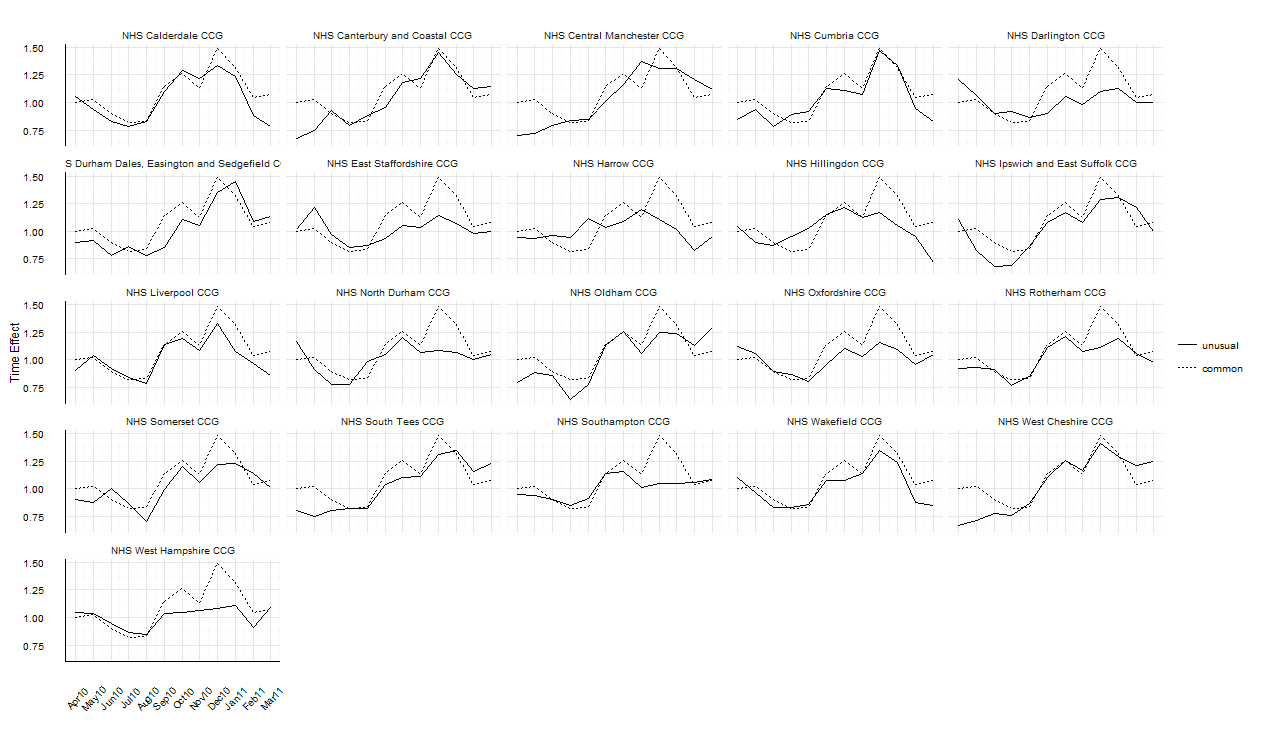
\includegraphics[height=6.8cm]{time_all.png}}}};
%  \pause
%  \node (img2) at (0,-1.7) {{\visible<2-2>{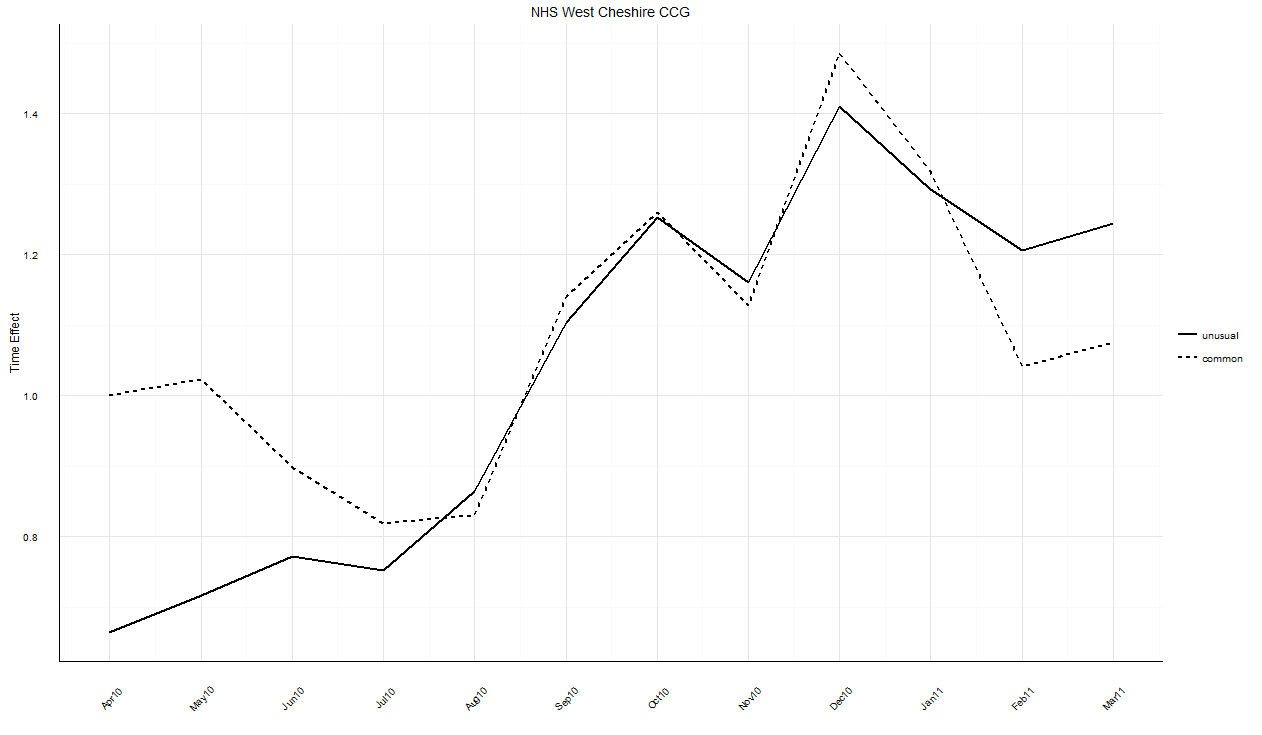
\includegraphics[height=5cm]{Cheshire.png}}}};
%  \pause
% \node (img3) at (0,-2.7){{\visible<3-3>{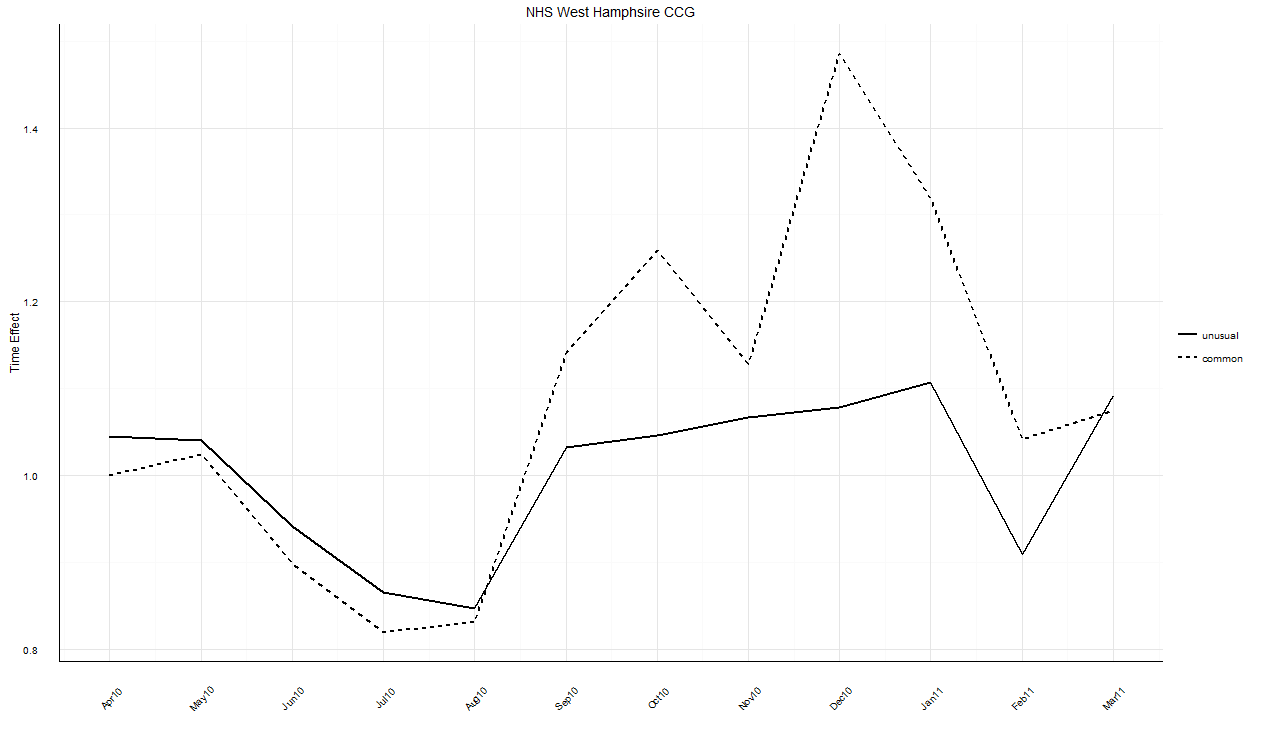
\includegraphics[height=5cm]{Hamphsire.png}}}};
% \pause
%  \node (img4) at (0,-3.7) {{\visible<4-4>{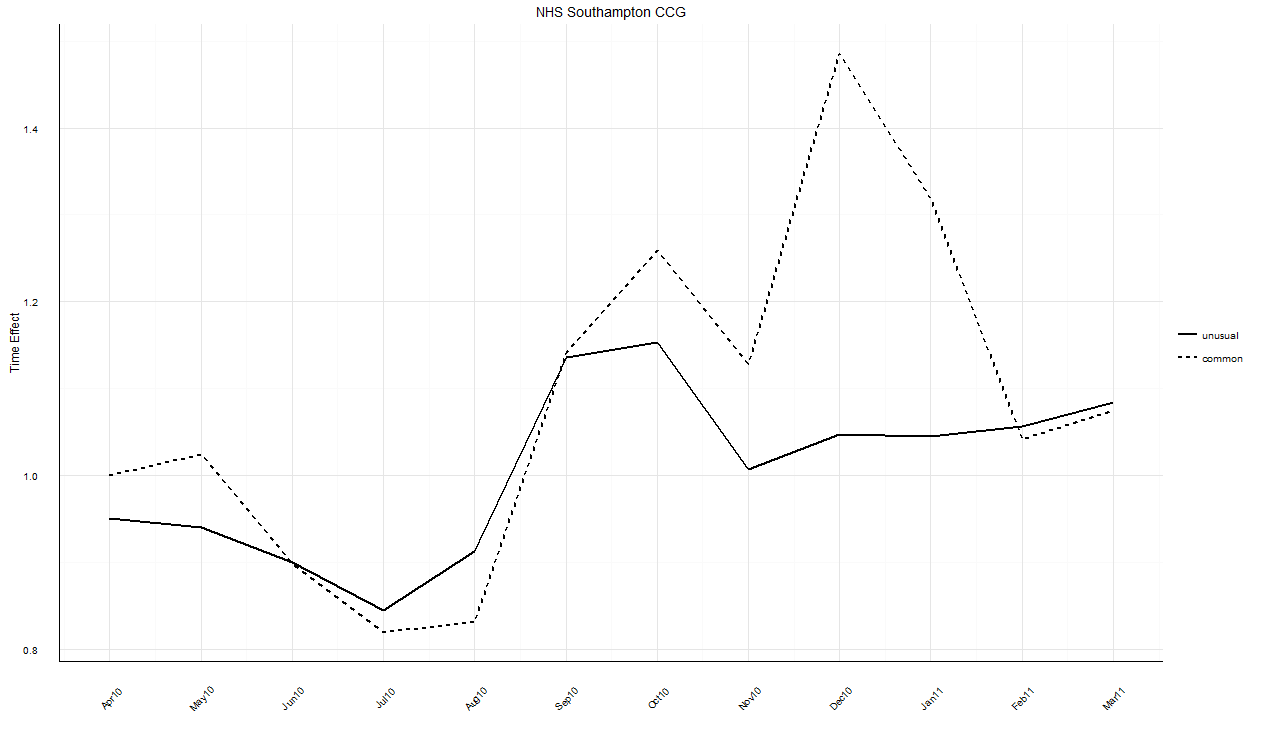
\includegraphics[height=5cm]{Southampton.png}}}};
% \pause
%  \node (img5) at (0,-4.7) {{\visible<5-5>{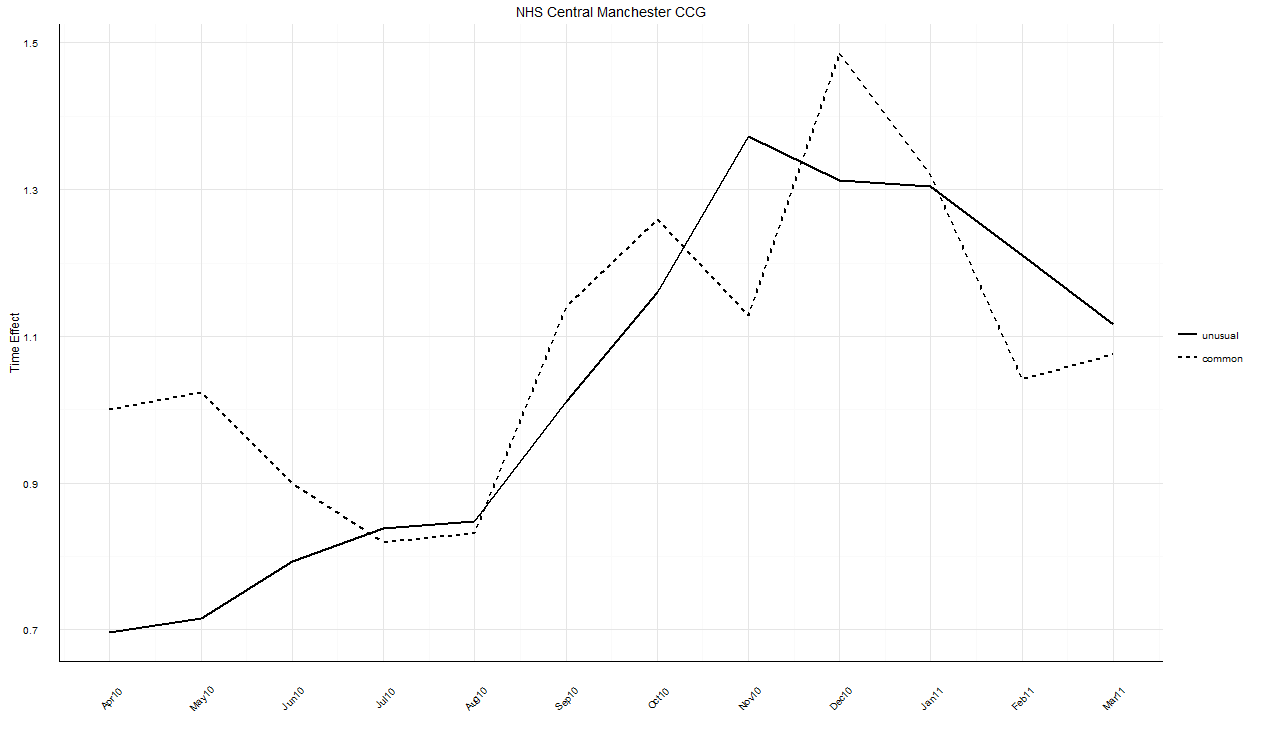
\includegraphics[height=5cm]{Manchester.png}}}};  
%\end{tikzpicture}
%\end{center}

\end{frame}

%%%%%%%%%%%%%%%%%%%%
%\subsection*{Results: Detected Areas}
%\begin{frame}{Results: Detected Areas as Unusual}
%
%\begin{columns}
%\begin{column}{0.5\linewidth}
%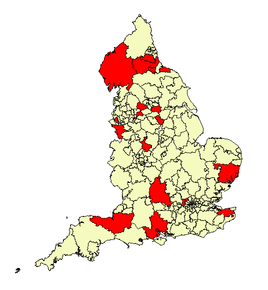
\includegraphics[scale=0.3]{outbreaks_map}
%\end{column}
%
%\begin{column}{0.5\linewidth}
%\begin{itemize}
%\item XX Detected areas as following an area-specific temporal trend
%\item Mostly isolated but also one cluster in the north of England
%\end{itemize}
%\end{column}
%\end{columns}
%
%\end{frame}
%%%%%%%%%%%%%%%%%%%%
\begin{frame}{Next Steps}
\begin{itemize}
\vfill\item Extend this framework to model several health outcomes.
\vfill\item  Create a user-friendly tool for people to disseminate this method.
\vfill\item Similar framework to be used to investigate trends in life expectancy (PHE funded).
\end{itemize}

\vspace{20pt}


\fontsize{7}{7}\selectfont{
Boulieri A, Bennett J, Blangiardo M, ``A Bayesian mixture modelling approach\\ for disease surveillance'', submitted to \textbf{Biostatistics}
}

\end{frame}


%%%%%%%%%%%%%%%%%%%%%%%%%%%%%%%%%%%%%%%%%%%%%%%%%%%%%%%%%%%%%%%%%
\section{Risk assessment}
\begin{frame}
\begin{center}
\vfill\fontsize{20}{20}\selectfont{Risk Assessment}\end{center}
\end{frame}

\begin{frame}
\frametitle{Health effects of polluted air: some estimates}
\vspace{-5pt}
\begin{itemize}
%\item \citet{forouzanfar2015}: Air pollution causes 5.5 million deaths worldwide per year (95\% CI: 5.1-5.9 million); \vspace{-1pt}
\item \citet{iarc2013}:  Outdoor air pollution is carcinogenic to humans; \vspace{-1pt}
\item \citet{whoeuro2006}: Outdoor  PM causes a reduction in life expectancy of average population by approximately a year in Europe;\vspace{-1pt}
\item \citet{who2016}: Outdoor PM$_{2.5}$ causes more than 3 million deaths per year worldwide; 92\% of the world's population lives in places where air quality levels exceed WHO limits.
 \end{itemize}

\begin{figure}[h]
 \centering
   \begin{tikzpicture}[overlay]
     \node at (-2,-1.6) {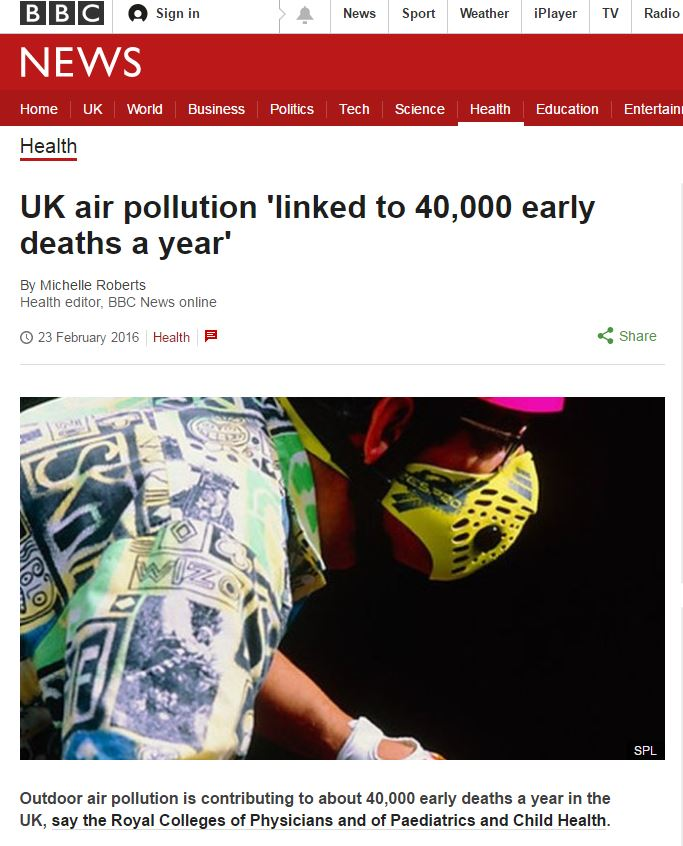
\includegraphics[width=3.4cm]{London40000.jpg}};
     \node at (2.3,-1.3) {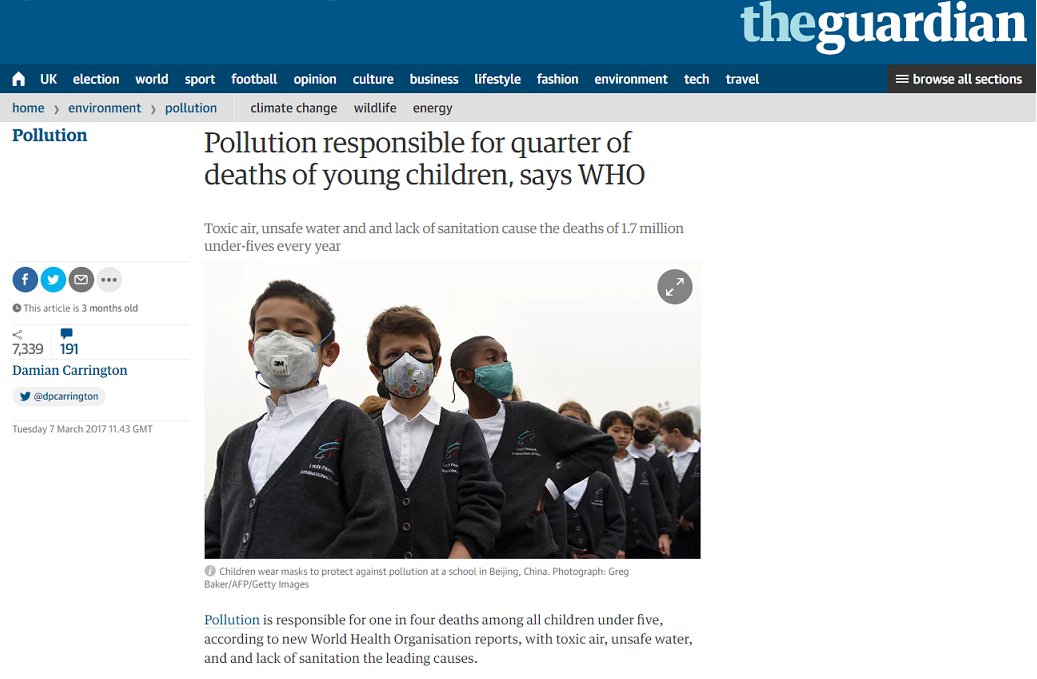
\includegraphics[width=6cm]{Airpoll2.png}};
  \end{tikzpicture}
\end{figure}
% \begin{figure}
%\hspace{-18pt}
%  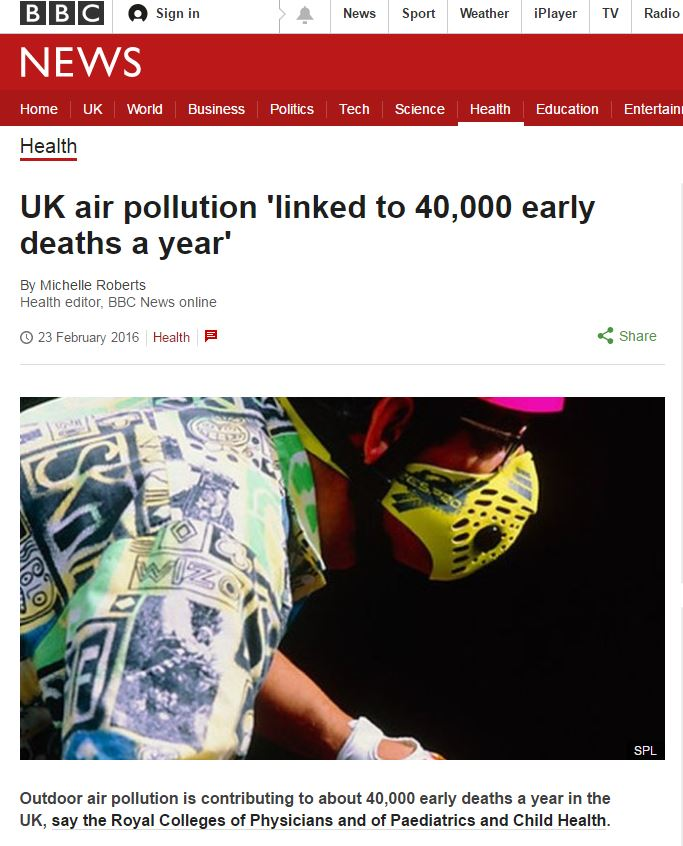
\includegraphics[width=3.7 cm]{London40000.jpg}
%\end{figure}

\end{frame}
%%%%%%%%%%%%%%%%%%%%%%%%%%%%%%%%%%%%%%%%%%%%%%%%%%%%%%%%%%%%%%%%%
\begin{frame}
\frametitle{Long-term effects vs Short-term}
\begin{itemize}
%\vfill\item Air pollution effects on health are typically classified be \textbf{long} or \textbf{short} term;
\vfill\item \alert{Long-term} considers averages of air pollution concentration and counts of outcomes (at individual level or) over small areas:
\begin{itemize}
\vfill\item typically air pollution data from exposure models (deterministic or more recently statistical);
\vfill\item important to account for area level confounders (e.g. population and area characteristics);
\vfill\item statistical approach is usually ecological regression.
\end{itemize}
\pause\vfill\item \alert{Short-term} considers the temporal variation in air pollution and evaluate the association with the temporal variation in health:
\begin{itemize}
\vfill\item typically air pollution data from monitoring stations (one or more);
\vfill\item important to account for seasonality and meteorological variables;
\vfill\item statistical modelling usually in a time-series framework.
\end{itemize}\end{itemize}
\end{frame}

%%%%%%%%%%%%%%%%%%%%%%%%%%%%%%%%%%%%%%%%%%%%%%%%%%%%%%%%%%%%%%%%%
\subsection{Residual confounding}
\begin{frame}
\begin{center}
\vfill\fontsize{20}{20}\selectfont{Risk Assessment: residual confounding}\end{center}
\end{frame}
%
%%%%%%%%%%%%%%%%%%%%%%%%%%%%%%%%%%%%%%%%%%%%%%%%%%%%%%%%%%%%%%%%%%%
%\begin{frame}
%\frametitle{Air pollution studies: Observational data}
%\begin{itemize}
%  \item \vfill Environmental epidemiological studies are observational:
%  \begin{itemize}
%\item \vfill Crucial evidence about real-world risks related to environmental and lifestyle exposures;
%\item \vfill Effects of risk factors or exposures typically depend on
%subject characteristics, which must be taken into account properly to
%avoid biases (\alert{confounder adjustment}).
%\end{itemize}
% \vfill\item Data sources: 
%\begin{itemize}
%\vfill\item  Cohort/surveys
%\begin{itemize}
%\vfill\item Contain detailed information on exposures / confounders;
%\vfill\item Might lack representativeness and statistical power.
%\end{itemize}
%\vfill\item Electronic health records
%\begin{itemize}
%\vfill\item Ensure high population representativeness and statistical power;
%\vfill\item Can be used at the aggregated level for disease surveillance;
%\vfill\item Only record a very limited set of information.
%\end{itemize}
%\end{itemize}\end{itemize}
%
%
%\end{frame}

%%%%%%%%%%%%%%%%%%%%%%%%%%%%%%%%%%%%%%%%%%%%%%%%%%%%%%%%%%%%%%%%%
\begin{frame}\frametitle{Air pollution and health in London}

\begin{itemize}
\vfill\item CHD\footnote{Coronary Heart Disease} admissions (Hospital Episode Statistics - HES), ICD codes I20 to I25. 
\vfill\item Analysis conducted at the middle super output area in London (MSOA - approx 6,500 individuals).
\vfill\item Concentration of PM$_{10}$ modelled through a land use regression ($X$).
\vfill\item Area level confounders: ethnicity and social deprivation ($\bm{C}$).
\end{itemize}

\begin{itemize}
\item Log linear model with spatially structured/unstructured random effects.
\end{itemize}
\begin{eqnarray*}
O_i &\sim& \text{Poisson}(\lambda_i \text{E}_i)\\
\text{log}(\lambda_i) &=& \alpha + {\color{red} \mathbf{X}_i^\top \boldsymbol{\beta_X}} + \boldsymbol{C}_{i}^\top\beta_{C} + u_i + v_i\end{eqnarray*}
\end{frame}
%%%%%%%%%%%%%%%%%%%%%%%%%%%%%%%%%%%%%%%%%%%%%%%%%%%%%%%%%%%%%%%%%
\begin{frame}
\frametitle{Air pollution and CHD hospital admissions in London: Results}

Data for 2001, PM$_{10}$ in quintiles

\vspace{10pt}
\begin{center}\begin{tabular}{lcc}
\hline
PM$_{10}$ & Posterior Mean & 95\%CI\\
\hline
<24.2 & 1.00 & ref\\
24.2-25.3 & 1.03 & 0.96-1.10\\
25.3-26.2 & 0.94 & 0.88-1.01\\
\color{red}{26.2-27.5} & \color{red}{0.88} & \color{red}{0.81-0.94}\\
\color{red}{>27.5}     & \color{red}{0.75} & \color{red}{0.70-0.81}\\
\hline
\end{tabular}\end{center}

%\pause \begin{center}\includegraphics[scale=0.4]{Figures/Arrow}\end{center}

\vspace{5pt} Several models investigated (spatial only, random effect only, spatial + random effect).
%Brian Reich, Effects of residual smoothing on the posterior of the fixed effects in disease-mapping models. Biometrics 2006%

\vspace{5pt} The negative association between air pollution and CHD hospital admissions points towards {\color{red} residual confounding}.

\end{frame}
%%%%%%%%%%%%%
\section{External information to deal with residual confounding}
\begin{frame}\frametitle{Using external information to deal with residual confounding}

The integration of data sources (registries, cohorts/surveys) has been investigated to deal with confounding issues at the individual level:

\begin{itemize}
\pause\item \citet{jackson_bayesian_2009}, \citet{molitor_using_2009} used Bayesian graphical models to build sub-models for each source of data that are then linked together in a coherent global analysis. 

$\rightsquigarrow$ Multiple imputation in a Bayesian framework, computationally intensive, works on a limited set of confounders.

\pause\item \citet{Mccandless2012} proposed to use the propensity score to link data sources at the individual level - application on water chlorination and birth weight using Millennium Cohort Study and Hospital Episode Statistics.
\end{itemize}

\pause\vspace{10pt} \begin{center}{\color{red} We develop a framework based on propensity score like indices for ecological (small area) studies.}\end{center}

\end{frame}
%%%%%%%%%%%%%%%%%%%%%%%%%%%%%%%%%%%%%%%%%%%%%%%%%%%%%%%%%%%%%%%%%%%%%%
\begin{frame}
\frametitle{Notation}
\begin{itemize}
\item \vfill Data measured only at \emph{geographical areas}, $i=1, \dots, N$
\begin{itemize}
  \item \vfill Outcome in analysis $O$.
  \item \vfill Exposure of interest $X$;
    \item \vfill Set of $Q$ covariates $\boldsymbol{C}$;

  \end{itemize}
\pause \item \vfill Data unmeasured at area-level, $i=1, \dots, N$
\begin{itemize}
\vfill \item Set of $K$ missing confounders $\boldsymbol{M}$.
\end{itemize}
\pause\item \vfill Data measured at individual-level within several geographical areas $i=1, \dots, S \in N$ (e.g. areas covered by a survey)
  \begin{itemize}
  \vfill \item Set of $K$ confounders $\boldsymbol{m}$, on $j=1,\dots, J$ subjects.
\end{itemize}
\end{itemize}

\pause\begin{block} {\centering Idea}
  \begin{itemize}
\item \vfill Use a hierarchical model that up-scales spatially-referenced individual data, $\boldsymbol{m}$, at ecological level, to provide latent (unmeasured) confounding factors, $\boldsymbol{M}$, for inclusion in the ecological health-effect model.
\item \vfill However, how to deal with areas where individual-level data are missing?
\end{itemize}
\end{block}
\end{frame}

%%%%%%%%%%%%%%%%%%%%%%%
\begin{frame}
\frametitle{Why is propensity score useful in areal-referenced studies?}
\centering $\small O_{i}\sim \text{Poisson}(E_{i} \lambda_{i})$
\begin{tabular}{cc}
\begin{minipage}{0.45\linewidth}
Areas with survey data
\begin{footnotesize}\begin{eqnarray*}
\log(\lambda_i) &=& \alpha +  X_i^\top {\color{red}\beta_X} + \boldsymbol{C}_{i}^\top\beta_{C}  + \\
				&&{\color{red} \boldsymbol{M}_{i}^\top \beta_{M}}  + u_{i} + v_{i}
\end{eqnarray*}
\end{footnotesize}
\end{minipage}

&
\hspace{3pt}

\begin{minipage}{0.45\linewidth}
\small Areas without survey data
\begin{footnotesize}\begin{eqnarray*}
\log(\lambda_i) &=& \alpha +  X_i^\top {\color{red}\beta_X} +  \boldsymbol{C}_{i}^\top\beta_{C} + \\
				&&{\color{red}?} + u_{i} + v_{i}
\end{eqnarray*}
\end{footnotesize}
\end{minipage}
\end{tabular}

%\pause\begin{tabular}{lc}
%\begin{minipage}{0.45\linewidth}
\begin{itemize}
  \item \vfill Without imputing the missing data only a partial spatial analysis can be carried out.\\
$\rightsquigarrow$ Not useful in a public health/surveillance perspective.
  \item \vfill Imputing several confounders raises methodological challenges and is computationally intensive.\\
$\rightsquigarrow$ {\color{red} Propensity Score} to provide dimension reduction.
\end{itemize}
\end{frame}

%%%%%%%%%%%%%%%%%%%%%%%%%%%%%%%%%%%%%%%%%%%%%%%%%%%%%%%%%%%%%%%%%%
\begin{frame}
\frametitle{Proposed approach}
\begin{enumerate} [{(1)}]
  \item \vfill Up-scaling the $\boldsymbol{m}$ to $\boldsymbol{M}$ ($i\in S$):
\begin{eqnarray*}
  m_{ikj} &\sim& \mbox{Bern}(M_{ik})\\
  g_{k}(M_{ik})&=& \eta_{k}+\xi_{ik} \qquad k=1,\ldots,K;
%\Bigg(\frac{1}{n_{i}}\sum_{s \in \partial_{i}}\xi_{ik},	 \frac{1}{n_{i}} \boldsymbol{\Gamma}_{i} \Bigg) \hspace{9pt}
\end{eqnarray*}
\begin{itemize}
  \item \vfill $\xi_{ik}$ are multivariate random effects;\\
%$\Longrightarrow$ They allow to model a spatial dependence across the geographical areal units while accommodating the correlation structure among the $K$ individual-level variables.     
  \item \vfill $\eta_{k}$ is confounder-specific fixed intercept and has a vague prior.
\end{itemize}
\pause  \item \vfill Ecological PS estimation (EPS) for non-missing areas ($i\in S$).
\begin{itemize}
\item \vfill For a binary exposure, we follow \citet{Mccandless2012}, that proposed the estimation of a partial PS for modelling missing confounders:
\begin{equation*}
\text{logit}(\text{Pr}(X_{i}=1 | \boldsymbol{C}_{i}, \boldsymbol{M}_{i} )) = \delta_{0} + \sum_{q} \delta_{q} C_{qi} + \underbrace{\alert{\sum_{k} \delta_{k}M_{ik}}}_{\alert{\text{EPS}}}
\end{equation*}

\begin{itemize}
\item $M_{ik}$ comes from the multilevel model.
\item Only one quantity has to be imputed where missing at the small area level.
\end{itemize}
\end{itemize}
\end{enumerate}
\end{frame}

%%%%%%%%%%%%%%%%%%%%%%%%%%%%%%%%%%%%%%%%%%%%%%%%%%%%%%%%%%%%%%%%%%
\begin{frame}
\frametitle{Proposed approach (cont.)}
 \begin{enumerate}[{(3)}]
\vfill \item Imputation model for missing areas:
\begin{equation*}
\text{EPS}_{i} \sim \text{Normal}(\eta + f(\boldsymbol{C}_i)+ \zeta_{i}, \sigma_{EPS}^2)
\end{equation*}
\begin{itemize}
\vfill \item $\zeta_{i}$ incorporates the spatial structure in the model.
\end{itemize}
\end{enumerate}

\pause\begin{enumerate}[{(4)}]
\item \vfill Health-effect model adjustment:\\
\begin{equation*}
\begin{split}
O_{i}\sim & \text{Poisson}(\text{E}_{i} \lambda_{i}), \hspace{9pt} i=1,\dots, N \\
\text{log}(\lambda_i) & = \beta_0 + \alert{X_{i}^\top \boldsymbol{\beta}_X} + \mathbf{C}_{i}^\top \boldsymbol{\beta}_C + \alert{h(\text{EPS}_i)} + u_{i} + v_{i}
\end{split}
\end{equation*}

\begin{itemize}
\vfill \item Data-driven function $h()$ to link EPS to the outcome-exposure analysis in order to minimise the model specification bias.
%\vfill \item Careful consideration of random effect structure to avoid collinearity with fixed effects.
\end{itemize}
\end{enumerate}
\end{frame}
%%%%%%%%%%%%%%%%%%%%%%%%%%%%%%%%%%%%%%%%%%%%%%%%%%%%%%%%%%%%
\begin{frame}\frametitle{To sum up}
\begin{figure}
\scalebox{.55}{\begin{tikzpicture}
%EPS estimation
%\draw(-14,1.5) node[align=center,circle,draw=none,fill=none,font=\sffamily\fontsize{9}{10}\selectfont,minimum width=.4cm,minimum height=.4cm](2){$\mu_t$};
\draw(-15.5,1.5) node[align=center,circle,draw=none,fill=none,font=\sffamily\fontsize{9}{10}\selectfont](M){Area\\level\\conf.\ $\bm{M}$};
\node[right=1 of M, circle,align=center,draw=black, fill=gray,font=\sffamily\fontsize{9}{10}\selectfont](EPS){EPS};
\node[right=0.5 of EPS, align=center,draw=none,fill=none,font=\sffamily\fontsize{9}{10}\selectfont](C){Area\\level\\conf.\ $\bm{C}$};
\node[above=0.5 of M, align=center,font=\sffamily\fontsize{9}{10}\selectfont](m){Indiv.\ level\\ conf.\ $\bm{m}$};
\node[above=0.4 of C, align=center,circle,draw=none,fill=none,font=\sffamily\fontsize{9}{10}\selectfont](X){Exposure\\$X$};
\node[below=0.5 of M, align=center,circle,draw=none,fill=none,font=\sffamily\fontsize{9}{10}\selectfont](SS1){Spatial\\ Structure\\ $\xi, \eta$};
%\node[right=1 of SS1, align=center,circle,draw=none,fill=none,font=\sffamily\fontsize{9}{10}\selectfont](delta){Regression\\ coefficients\\$\boldsymbol{\delta}$};
%\path[line](FB)()% Rounded rectangles
\draw[rounded corners=15pt,thick] (-16.8,-1.6) rectangle ++ (7.1,6.2) node[xshift=-5.5cm, yshift=0.1cm]{\fontsize{6}{7}\selectfont \sffamily Survey areas ($i \in S$)} ;
%Eq 2.1
\draw[rounded corners=15pt,dotted,thick] (-16.4,-1.45) rectangle ++ (2.2,5.8);
%Eq 2.2
\draw[rounded corners=15pt,dotted,thick] (-13.9,-1.45) rectangle ++ (3.8,5.8);
% Arrows
\draw [->,>=latex,shorten >=-2pt,auto,node distance=2pt,thin] (M.north) -- (m.south);
\draw [->,>=latex,shorten >=-6pt,shorten <=-10pt,auto,node distance=2pt,thin] (SS1.north) -- (M.south);
\draw [->,>=latex,shorten >=-12pt,auto,node distance=2pt,thin] (C.north) -- (X.south);
\draw [->,>=latex,shorten >=-8pt,shorten <=2pt,auto,node distance=2pt,thin] (EPS.60) -- (X.south west);
\draw [->,>=latex,shorten >=2pt,shorten <=-5pt,auto,node distance=2pt,thin] (M.east) -- (EPS.west);
%\draw [->,>=latex,shorten >=-6pt,auto,node distance=2pt,thin] (delta) to [out=0,in=10, looseness=0.5](X);
%\draw [->,>=latex,shorten >=2pt,shorten <=-5pt,auto,node distance=2pt,thin] (FB.north) -- (EPS.west);
%\draw[-,>=latex,shorten >=6pt,shorten <=-10pt,auto,node distance=2pt,thin, dashed] (FB) -- (-14.05, 1.7);
% EPS imputation
\draw[fill=gray] (-7.7,2.05) rectangle (-6.6,0.92);
\node[right=5 of EPS, align=center,circle,draw=black, fill=gray,font=\sffamily\fontsize{9}{10}\selectfont](EPS2){EPS};
\node[above=0.8 of EPS2, align=center,font=\sffamily\fontsize{9}{10}\selectfont](C2){Area\\level\\conf.\ $\bm{C}$};
\node[right=1 of EPS2, align=center,font=\sffamily\fontsize{9}{10}\selectfont](X2){Exposure\\$X$};
\node[below=0.8 of EPS2, align=center,circle,draw=none,fill=none,font=\sffamily\fontsize{9}{10}\selectfont](SS3){Spatial\\ Structure \\ $\zeta$};
%% Arrows
\draw [->,>=latex,shorten >=5pt,shorten <=-10pt,auto,node distance=2pt,thin] (SS3.north) -- (EPS2.south);
\draw [->,>=latex,shorten >=3pt,auto,node distance=2pt,thin] (X2.west) -- (EPS2.east);
\draw [->,>=latex,shorten >=5pt,auto,node distance=2pt,thin] (C2.south) -- (EPS2.north);

% EPS adjustment
%\draw[fill=gray, dashed] (-6.2,2.15) rectangle (-7.7,0.75);
\node[below=5 of EPS2, align=center,circle,draw=none,fill=none,font=\sffamily\fontsize{9}{10}\selectfont](O){Health\\Outcome\\ $O$};
\node[right=1 of O, align=center,circle,draw=none,fill=none,font=\sffamily\fontsize{9}{10}\selectfont](SS4){Spatial\\ Structure\\ $u, v$};
\node[below=0.8 of SS3, align=center,circle,draw=none,fill=none,font=\sffamily\fontsize{9}{10}\selectfont](E){$E$};

% Rounded rectangles

%% Arrows
\draw [->,>=latex,shorten >=-7pt,shorten <=2pt,auto,node distance=2pt,thin] (EPS2.west) to [out=-190,in=-195, looseness=0.35] (O);
\draw [->,>=latex,dashed,shorten >=2pt,shorten <=-5pt,auto,node distance=.3pt,line width=.2mm] (O.west) to [out=-190,in=-190, looseness=0.42] (EPS2);
\draw [->,>=latex,shorten >=-5pt,auto,node distance=2pt,thin] (SS4.west) -- (O.east);
\draw [->,>=latex,shorten >=-5pt,auto,node distance=2pt,thin] (C2.east) to [out=0,in=20, looseness=1.15] (O);
\draw [->,>=latex,shorten >=-10pt,auto,node distance=2pt,thin] (X2.240) -- (O.70);
\draw [->,>=latex,shorten >=-10pt,auto,node distance=2pt,thin] (E.south) -- (O.north);

% Rounded rectangles
\draw[rounded corners=15pt,thick] (-8.7,-6.5) rectangle ++ (5.5,11.1) node[xshift=-4.0cm, yshift=0.1cm]{\fontsize{6}{7}\selectfont \sffamily All areas ($i \in N$)};
%Eq 2.3-2.4
\draw[rounded corners=15pt,dotted,thick] (-8.4,-1.5) rectangle ++ (5,5.9);
%Eq 2.5
\draw[rounded corners=15pt,dotted,thick] (-8.4,-6) rectangle ++ (5,4);

\pause \node[above=2 of X, red, align=left,draw=none,fill=none, font=\sffamily\fontsize{12}{12}\selectfont](text1) {Uncertainty on the parameters is propagated throughout the model};
\pause \node[left=0.5 of M, red,align=left,rectangle,draw,fill=none, font=\sffamily\fontsize{10}{10}\selectfont](text2) {$\rightarrow$From the estimates\\ of ${\mathbf M}$\\ into the\\ EPS estimation};
\pause \node[right=1.1 of X2, red,align=left,rectangle,draw,fill=none, font=\sffamily\fontsize{10}{10}\selectfont] (text3) {$\rightarrow$ From the\\ EPS imputation into\\ the analysis model};
\pause \node[below=3 of EPS, red,align=left,rectangle,draw,fill=none, font=\sffamily\fontsize{10}{10}\selectfont] (text4) {Feedback from $X$ to $M$ is prevented};
\pause \node[below=2 of text3, red,align=left,rectangle,draw,fill=none, font=\sffamily\fontsize{10}{10}\selectfont] {Feedback from $O$\\ to EPS\\ is allowed};
\end{tikzpicture}}
 \end{figure}

\vspace{-15pt}
\hrulefill

%\fontsize{8}{8}\selectfont{Ziegler C, et al. (2013), Biometrics; 69(1):263-273.}\\ 
%\fontsize{8}{8}\selectfont{Kenward M and Carpenter J. (2007), Statistical Methods in Medical Research; 16(3):199-218.}
\end{frame}

%%%%%%%%%%%%%%%%%%%%%%%%%%%%%%%%%%%%%%%%%%%%%%%%%%%%%%%%%%%
%\begin{frame}\frametitle{London air pollution and hospitalisations for CHD}
%Analysis performed on 6044 middle layer super output areas (MSOAs).
%\begin{itemize}
%\vfill\item Outcome: Hospitalisation for CHD (ICD10: I20-I25) from Hospital Episode Statistics registry.
%\vfill\item Exposure: PM$_{10}$ from land use regression model.
%\vfill\item Ecological confounders: Deprivation index and ethnicity.
%\vfill\item Individual confounders: Health Survey for England (HSfE) data collected on 95,467 individuals.
%\begin{itemize}
%\vfill\item Thirteen confounders which could
%potentially bias the relationship between air pollution and CHD hospital admissions:
%education, smoking, passive smoking, drinking, overweight, obesity, mental illness, regular
%exercise (sports), diabetes, high blood pressure, vitamin taken, high cholesterol and table
%salt intake.
%\vfill\item MSOAs with no individuals were treated as missing.
%\end{itemize}
%\end{itemize}
%\end{frame}

%%%%%%%%%%%%%%%%%%%%%%%%%%%%%%%%%%%%%%%%%%%%%%%%%%%%%%%%%%%%%%%%%
\begin{frame}\frametitle{London air pollution and CHD hospitalisations: adjusting for EPS}
Association between CHD and exposure to PM$_{10}$ dichotomised using a cut-off of 25$\mu g/m^{3}$.

\vspace{5pt} Individual level data obtained from the Health Survey of England 1994-2001. 13 potential confounders were considered covering smoking, drinking, BMI, physical activity, diet.
\scalebox{.7}{\begin{tikzpicture}
\node[anchor=south west,inner sep=0] (image) at (-3,1) {\includegraphics[scale=0.25]{C6_Forest_1_ldn_pm10.png}};
\node[align=center,black, fill=white](M) at (-2,5) {\fontsize{8}{8}\selectfont \sffamily Naive case (ignoring $\boldsymbol{M}$)};
\node[below=0.9 of M, align=center,black, fill=white](Adj) {\fontsize{8}{8}\selectfont \sffamily EPS adjustment};
\node[below=0.9 of Adj, align=center,black, fill=white](Imp) {\fontsize{8}{8}\selectfont \sffamily EPS imputation};
\node[above=1 of M, align=center,white, fill=white](nothing) {blablablablablablabla};
\pause\node[right=4 of M, align=center,black, fill=white](M1) {\fontsize{8}{8}\selectfont \sffamily Negative association,\\
\fontsize{8}{8}\selectfont \sffamily suggesting residual confounding.};
\pause\node[below=0.5 of M1, align=center,black, fill=white](Adj1) {\fontsize{8}{8}\selectfont \sffamily Positive association,\\ \fontsize{8}{8}\selectfont \sffamily \color{red} posterior probability 98.4\%.};
\pause\node[below=0.5 of Adj1, align=center,black, fill=white](Imp1) {\fontsize{8}{8}\selectfont \sffamily Positive association\\ \fontsize{8}{8}\selectfont \sffamily more noise due to\\ \fontsize{8}{8}\selectfont \sffamily imputation,\\ \fontsize{8}{8}\selectfont \sffamily \color{red} posterior probability 85.3\%.};
\end{tikzpicture}}

\vspace{10pt}\fontsize{7}{7}\selectfont{Wang Y, et al. (2017), Using ecological propensity score to adjust for missing confounders in small area studies; \textbf{Biostatistics} (accepted).}\\ 
\end{frame}

%%%%%%%%%%%%%%%%%%%%%%%%%%%%%%%%%%%%%%%%%%%%%%%%%%%%%%%%%%%%%%%%%
\begin{frame}
\frametitle{Next steps}
\begin{itemize}
  \item \vfill Extension of the framework for a multi-categorical or continuous exposure.
%  \item \vfill The individual-scale variables may present different degree of dependence.
  %\item \vfill the exposure and the individual-scale variables may be geographically distributed hence spatially correlated;
  \item \vfill Model to account for nonlinearity between the individual level confounders and the outcome.
\item \vfill From spatial to spatio-temporal dimension.
\end{itemize}

\end{frame}
%%%%%%%%%%%%%%%%%%%%%%%%%%%%%%%%%%%%%%%%%%%%%%%%%%%%%%%%%%%%%%%%%
%%%%%%%%%%%%%%%%%%%%%%%%%%%%%%%%%%%%%%%%%%%%%%%%%%%%%%%%%%%%%%%%%
\subsection{Correlated Exposures}
\begin{frame}
\begin{center}
\vfill\fontsize{20}{20}\selectfont{Risk Assessment: correlated exposures}\end{center}
\end{frame}
%
%%%%%%%%%%%%%%%%%%%%%%%%%%%%%%%%%%%%%%%%%%%%%%%%%%%%%%%%%%%%%%%%%%

%\subsection{Correlated exposures}
\begin{frame}
\frametitle{From a single to a multi-pollutant approach}
\begin{itemize}
\item The quantification of the impact of air pollution on population health has been historically undertaken through a \textbf{single pollutant approach}. \vspace{-1pt}
\item This is mainly due to:
\begin{itemize}
%\item measurement and source complexities which have limited the development of statistically robust multi-pollutant models; \vspace{-1pt}
\item regulatory strategies of air quality management which have addressed a single pollutant at a time. \vspace{-1pt}
 \end{itemize}
 \end{itemize}
 \vspace{3pt}
\pause \alert{However}, the air we breathe is a mixture and:
\begin{itemize}
 \item It is unlikely that all parts of the air pollution mix are equally harmful;\vspace{-1pt}
 \item It is clear that the effect estimates can be affected by correlation, measurement error and exposure misclassification (locally varying vs regional pollutants).
\end{itemize}
 \vspace{3pt}
Therefore, we need new/revised statistical methods and approaches for a \alert{multi-pollutant approach} (e.g. \citealt{cull2015} and \citealt{molitor2016}).
\end{frame}
%%%%%%%%%%%%%%%%%%%%%%%%%%%%%%%%%%%%%%%%%%%%%%%%%%%%%%%%%%%%%%%%%%
\begin{frame}
\frametitle{Multi-pollutant approach so far}
\begin{itemize}
\vfill\item Air quality indexes (Daily Air Quality Index in the UK)\\
$\rightarrow$ typically used by governments;\\
$\rightarrow$ easy to build and to communicate to the public.
\vfill\item Bayesian Kernel Machine Regression (\citealt{Bobb:2015})\\
$\rightarrow$ the pollutants are included in the model through a smooth function represented using a kernel;\\
$\rightarrow$ authors found that Gaussian kernel outperformed linear and ridge regression kernels.
\vfill\item Dirichlet process mixture model (profile regression, \citealt{PIRANI201556})\\
$\rightarrow$ days are clustered based on their concentration profiles;\\
$\rightarrow$ concentration and health outcome are modelled jointly.
\end{itemize}
\end{frame}
%%%%%%%%%%%%%%%%%%%%%%%%%%%%%%%%%%%%%%%%%%%%%%%%%%%%%%%%%%%%%%%%%%
\begin{frame}
\frametitle{Another way forward}
We propose the use of a hierarchical Bayesian time-series approach which is formed by two linked components:
\begin{itemize}
\vfill\item A \textbf{pollutant component} which estimates the true `latent' concentration values;
\vfill\item A \textbf{health component} which links the estimated concentration to the health outcome;\\
\vfill\item The two components are \alert{jointly modelled};\\
\vfill\item The modelling framework allows to estimate a health effect for each pollutant.
\end{itemize}
\end{frame}
%%%%%%%%%%%%%%%%%%%%%%%%%%%%%%%%%%%%%%%%%%%%%%%%%%%%%%%%%%%%%%%%%%%
\begin{frame}
\frametitle{Data description}
\begin{itemize}
\item Daily measurements of five regulated pollutants and the number of particles present in any given volume of air (PCN) available from a monitoring site in North Kensington for 2011-2012.
\item Daily count of mortality for cardio-vascular disease (ICD-10, Chapter I) available for the same period.

\end{itemize}
\begin{footnotesize}
\begin{tabular}{|l|c|ccccc|c|}
\hline
& Number & \multicolumn{5}{c|}{Percentiles} & \\
& of Days & 10th & 25th & 50th & 75th & 90th  & IQR\\
\hline
Mortality & 731 & {\color{white}.} 28 & {\color{white}.}  32 & {\color{white}.}  37 & {\color{white}.}  42 & {\color{white}.}  47 & {\color{white}.}  10\\
\emph{Meteorological data}: & & & & & & & \\
Temperature ($^\circ C$) & 731 & {\color{white}.} 5.1 & {\color{white}.} 8.0 & 11.7 & 15.5 & 18.1 & {\color{white}.}7.4\\
Relative Humidity (\%) & 731 & 61.6 & 69.6& 78.0& 84.2 &88.5 & 14.5\\
\emph{Pollutants}: & & & & & & & \\
$\quad$ CO ($mg/m^3$) & 715 & {\color{white}.} 0.1 &{\color{white}.} 0.2 & {\color{white}.} 0.2 & {\color{white}.} 0.3& {\color{white}.} 0.4& {\color{white}.} 0.1\\
$\quad$ NO$_2$ ($\mu g/m^3$) & 706 & 18.2 & 23.2& 33.3 & 46.9 & 57.9 & 23.6\\
$\quad$ O$_3$ ($\mu g/m^3$) & 695 & 11.4 & 24.3 & 39.1 & 51.1 & 64.9 & 26.8\\
$\quad$ SO$_2$ ($\mu g/m^3$) & 717 & {\color{white}.} 0.0 & {\color{white}.} 0.4 & {\color{white}.} 1.8 & {\color{white}.} 2.6 & {\color{white}.} 3.6 & {\color{white}.} 2.2\\
$\quad$ PM$_{2.5}$ ($\mu g/m^3$) & 730 &  {\color{white}.} 5.0  & {\color{white}.} 6.0  & {\color{white}.} 9.0 & 14.0  &25.0 & {\color{white}.} 8.0\\
$\quad$ PCN ($p/mm^3$)& 636& {\color{white}.} 7.8 & {\color{white}.} 9.7 &12.1& 14.9 & 17.9 & {\color{white}.} 5.2 \\
\hline
\end{tabular}\end{footnotesize}

\end{frame}
%%%%%%%%%%%%%%%%%%%%%%%%%%%%%%%%%%%%%%%%%%%%%%%%%%%%%%%%%%%%%%%%%%%
\begin{frame}
\frametitle{H2M: pollutant component}
\begin{itemize}
\vfill\item We specify $X_{pt}$ as the measured (standardised) concentration level of pollutant $p$ ($p=1,...,P=6$) on day $t$ ($t=1,...,T=731$) from the monitoring site:
\vspace{10pt}\begin{eqnarray*}
X_{pt}&\sim& N(\mu_{pt}, \sigma^2_p)\\
\mu_{pt}&=& \gamma_{0p} + \sum_j \gamma_{jp}\text{z}_{jt} + \theta_{pt} \hspace{10pt}\text{\textbf{True} (latent) concentration model}
\end{eqnarray*}
\vfill\item $\mathbf{z}_t$ - meteorological variables:\\
$\Rightarrow$ Evidence of non-linear relationship with the pollutant levels - inclusion of linear and quadratic terms.
\end{itemize}
\end{frame}
%%%%%%%%%%%%%%%%%%%%%%%%%%%%%%%%%%%%%%%%%%%%%%%%%%%%%%%%%%%%%%%%%%
\begin{frame}
\frametitle{H2M: pollutant component - $\mathbf{\theta}$}
\begin{itemize}
\vfill\item $\{\theta_{1t}, \ldots, \theta_{Pt}\}$ accounts for the residual temporal effects and for the correlation among pollutants
\end{itemize}
\begin{eqnarray*}
(\theta_{1t},...,\theta_{Pt})^\top  \sim \text{MVN}\left((\theta_{1,t-\ell},...,\theta_{P,t-\ell})^\top , \Sigma_P\right)
\end{eqnarray*}
\begin{itemize}
\vfill\item  $t-\ell$ provides the temporal lag of $\ell$ days for the $t$-th day;
\vfill\item The diagonal of the covariance matrix of the errors $\Sigma_P$ allows each pollutant to have a different amount of temporal dependence;
\vfill\item The off-diagonals represent the temporal dependence between the pollutants.
\end{itemize}
\end{frame}
%%%%%%%%%%%%%%%%%%%%%%%%%%%%%%%%%%%%%%%%%%%%%%%%%%%%%%%%%%%%%%%%%%
\begin{frame}
\frametitle{H2M: health component}
\begin{itemize}
\item The second model component links the \textbf{true} concentration $\mu_{pt}$ to the health outcome
\end{itemize}
\begin{eqnarray*}
O_t &\sim& \text{Poisson}(\lambda_t E)\\
\log(\lambda_{t})&=& \beta_0 + \sum_p \beta_p \mu_{p(t-1)} + \sum_i s(v_{ti}, \psi_i) + \delta_{I_t} + \epsilon_t
\end{eqnarray*}

\begin{itemize}
\item $\lambda_t$ represents the relative risk of CVD death on day $t$ compared to the average;
\item we consider lag $\ell=1$ (same as \citealt{Atkinson:2016});
\item $\boldsymbol{\beta}$ are the pollutant effects on CVD mortality;
\item $\epsilon_t$ is an overdispersion parameter;
\item $ s(v_{ti}, \psi_i)$ is modelled through a low-rank thin plate spline:	
\end{itemize}
\[s(v_{ti}, \psi_{i})= \alpha_{i} v_{ti} + \sum_{k=1}^{K_{i}} b_{ki} | v_{ti}-\kappa_{ki}|^3
\]
\end{frame}
%%%%%%%%%%%%%%%%%%%%%%%%%%%%%%%%%%%%%%%%%%%%%%%%%%%%%%%%%%%%%%%%%%%
%\begin{frame}
%\frametitle{H2M: Graphical representation}
%\begin{itemize}
%\item Pollutant and health components are jointly modelled\\
%$\Rightarrow$ Uncertainty on $\mu_{pt}$ is fed forward\\
%$\Rightarrow$ Information on the outcome $y_{t}$ is fed back
%\end{itemize}
%\begin{tabular}{cc}
%\begin{minipage}{0.5\textwidth}
%\centering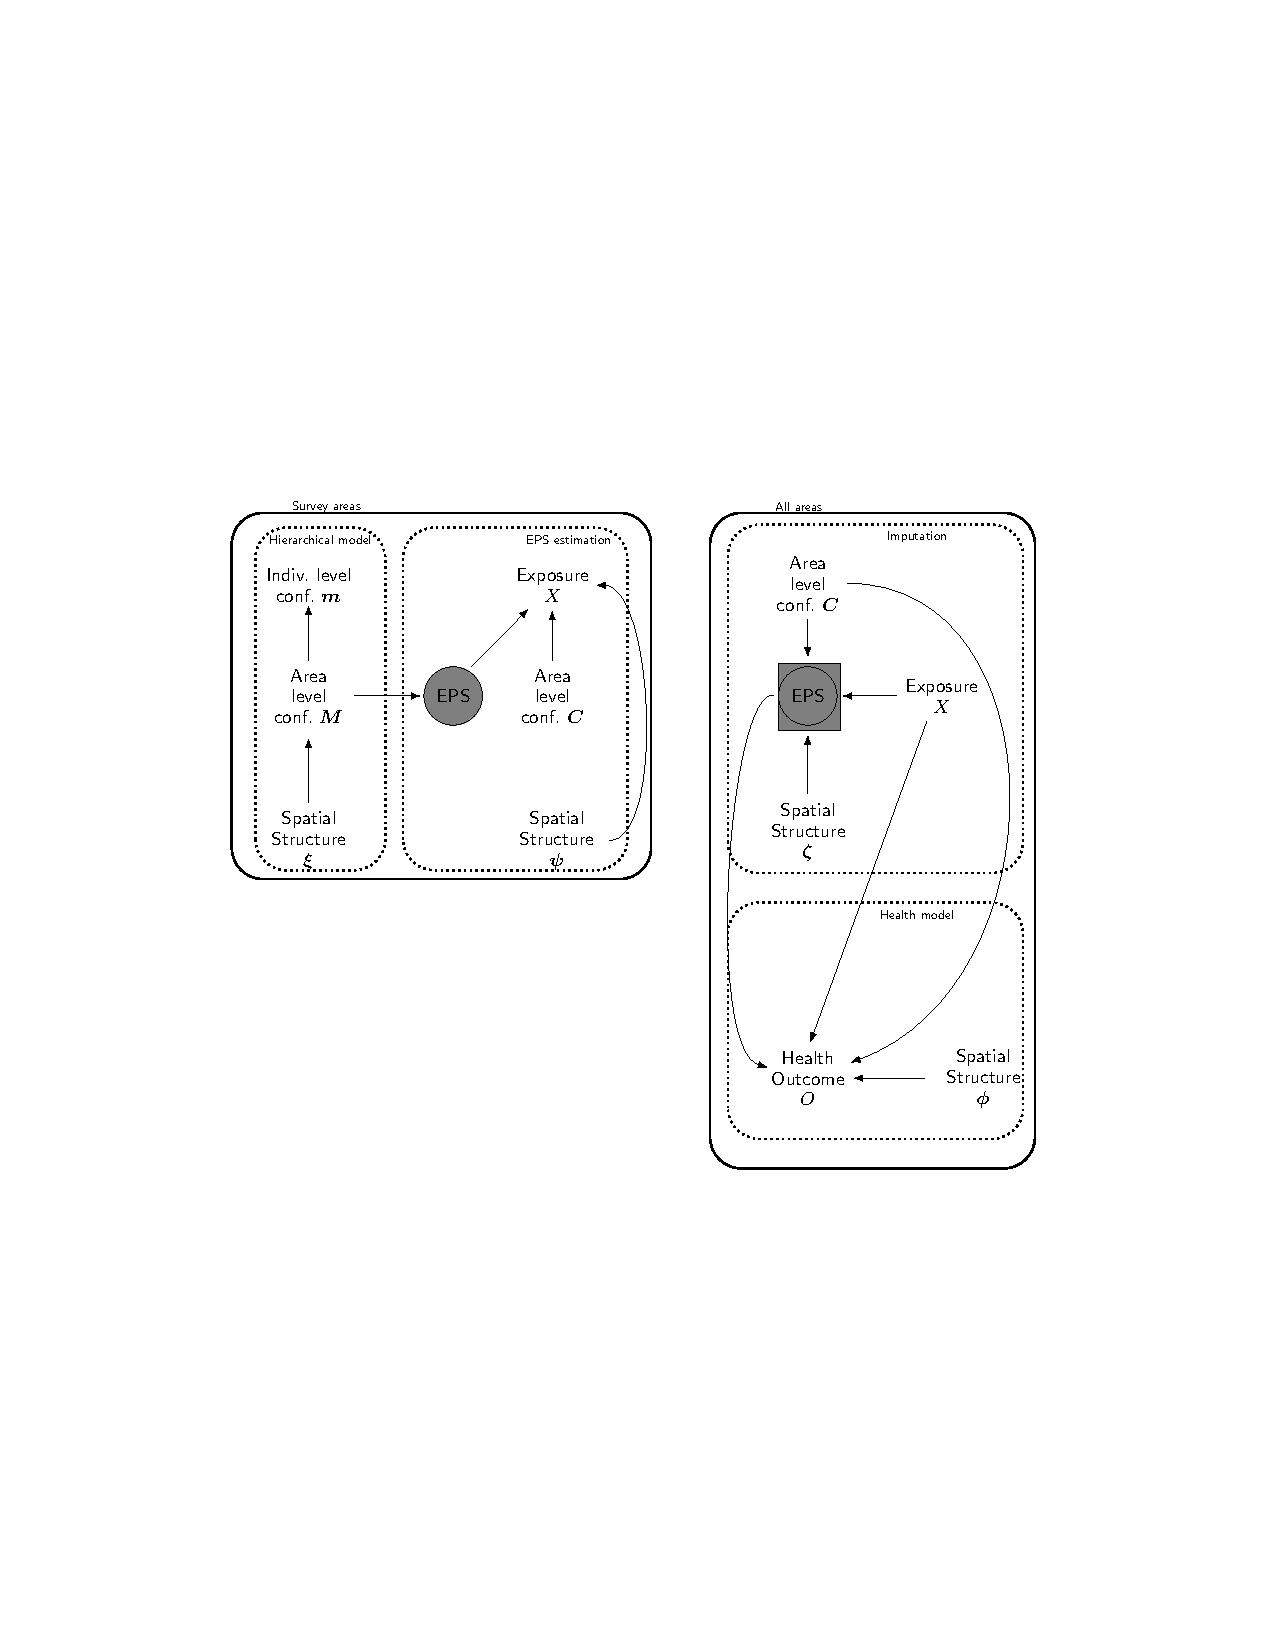
\includegraphics[scale=0.8]{GraphicalModel.pdf}
%\end{minipage}
%&
%
%\begin{small}\begin{minipage}{0.5\textwidth}
%\begin{itemize}
%\item $\Sigma_P \sim \text{IW}(D,d)$ with $d=P$
%\item Regression coefficients are $\text{N}(0,10^5)$
%\item Measurement error sd $\sigma_p\sim \text{U}(0,100)$
%\item Coefficients for the basis functions: $b_{ki} \sim \text{N}(0,\sigma^2_{b_i})$;\\ $1/\sigma^2_{b_i}\sim \text{Ga}(1,0.01)$
%\end{itemize}
%\end{minipage}\end{small}
%\end{tabular}
%\end{frame}
%%%%%%%%%%%%%%%%%%%%%%%%%%%%%%%%%%%%%%%%%%%%%%%%%%%%%%%%%%%%%%%%%%%%
%\begin{frame}
%\frametitle{Simulation study: setting}
%We consider (i) 6 pollutants, (ii) 2000 days, (iii) degree of correlation among pollutants varying between -0.6 and 0.8.
%
%We generate:
%\begin{enumerate}
%\item true pollutant concentration through $\mu_{pt} \sim \text{N}(\mu_{p(t-1)}, \Sigma_P)$
%\item measured concentration through $x_{pt} \sim \text{N}(\mu_{pt},0.1)$
%\item number of daily health events through a Poisson
%\item $\beta_p$ equal to -0.2, 0 or 0.2.
%\item Joint vs two-stage model
%\end{enumerate}
%
%\vspace{10pt} We estimate our H2M framework and compare it against a simpler model which include the pollutant concentration with measurement error (ME):
%
%\begin{eqnarray*}
%y_t &\sim& \text{Poisson}(\lambda_{t}E)\nonumber\\
%\log(\lambda_{t})&=& \beta_0 + \sum_p \beta_p x_{p(t-1)} + \epsilon_t
%\end{eqnarray*}
%\end{frame}
%%%%%%%%%%%%%%%%%%%%%%%%%%%%%%%%%%%%%%%%%%%%%%%%%%%%%%%%%%%%%%%%%%%
%\begin{frame}
%\frametitle{Simulation study: results}
%\begin{tabular}{cc}
%\begin{minipage}{0.4\textwidth}
%\begin{itemize}
%\item Bias and RMSE are substantially reduced for H2Ms;
%\item Coverage improves in H2Ms;
%\item Uncertainty is larger for H2Ms.
%\end{itemize}
%\end{minipage}
%
%&
%
%\begin{minipage}{0.7\textwidth}
%\begin{center}
%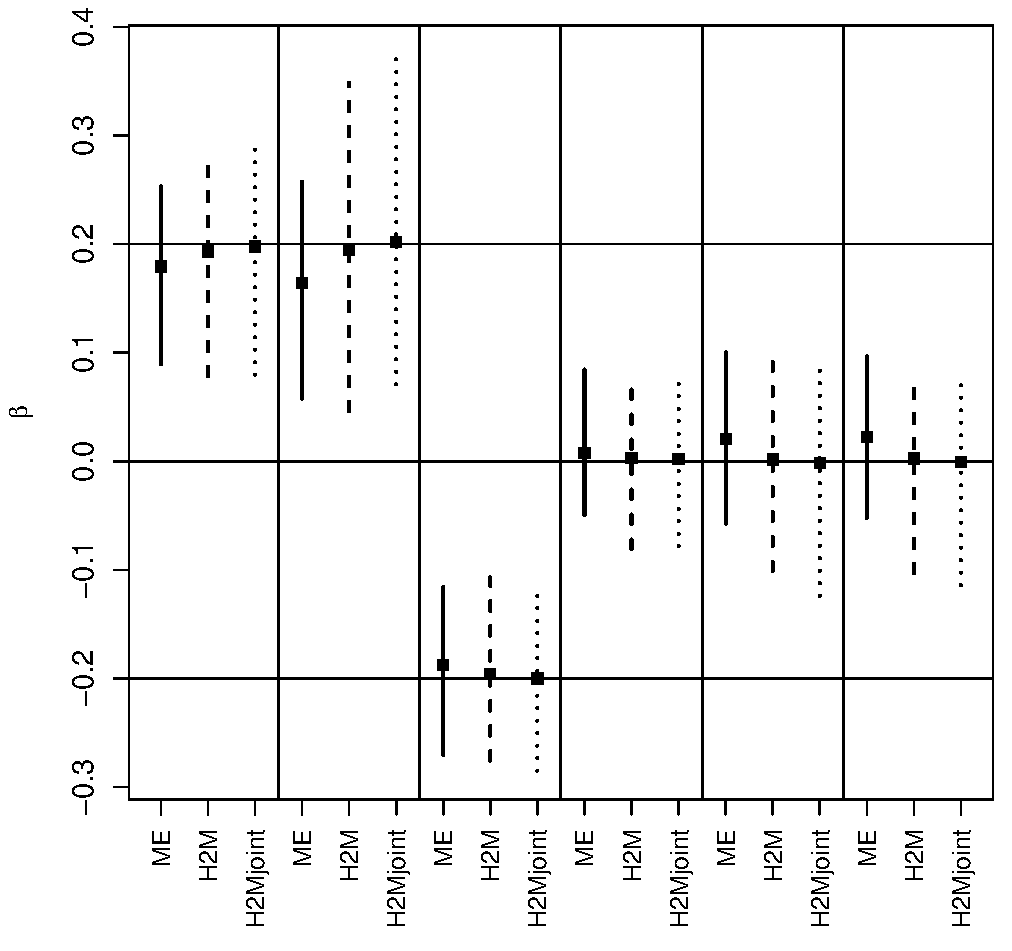
\includegraphics[scale=0.35]{ModelComparison}
%\end{center}
%\end{minipage}
%\end{tabular}
%
%\vspace{2pt}\fontsize{7}{7}\selectfont{\hspace{-10pt}\begin{tabular}{|c|p{0.8cm}p{0.8cm}p{0.8cm}|p{0.7cm}p{0.8cm}p{0.7cm}|p{0.5cm}p{0.8cm}p{0.5cm}|}
%\hline
%& \multicolumn{3}{|c}{Bias}	& \multicolumn{3}{c}{RMSE} & \multicolumn{3}{c|}{95\% CI coverage}\\
%\hline
%& &  & & & & & & & \\
%		  &	\hspace{3pt}ME		&H2Mj	& H2M & \hspace{3pt}ME	&H2Mj	& H2M & 	ME	&H2Mj & H2M\\
%& &  & & & & & & & \\
%
%$\beta_1$ & -0.021 & -0.002 & -0.007 & 0.003 & 0.002 & 0.002 &  65 & 93 & 92\\
%$\beta_2$ & -0.036 & \hspace{3pt}0.002 & -0.006 & 0.004 & 0.004 & 0.005 &  53 & 97 & 97\\
%$\beta_3$ & \hspace{3pt}0.013  & \hspace{3pt}0.000 & \hspace{3pt}0.004 & 0.003 & 0.002 & 0.004 &  71 & 97 & 92\\
%$\beta_4$ &\hspace{3pt}0.008  & \hspace{3pt}0.002 & \hspace{3pt}0.003 & 0.001 & 0.001 & 0.002 &  77 & 99 & 98\\
%$\beta_5$ & \hspace{3pt}0.021 & \hspace{1pt}-0.001 & \hspace{3pt}0.002 & 0.002 & 0.002 & 0.002 &  61 & 94 & 95\\
%$\beta_6$ & \hspace{3pt}0.022 &\hspace{1pt}-0.001 & \hspace{3pt}0.002 & 0.002 & 0.002 & 0.002 &  65 & 99 & 97\\
%\hline
%\end{tabular}
%}
%\end{frame}
%%%%%%%%%%%%%%%%%%%%%%%%%%%%%%%%%%%%%%%%%%%%%%%%%%%%%%%%%%%%%%%%%%%
%%\begin{frame}
%%\frametitle{Simulation study: dis-joining the model}
%%\begin{itemize}
%%\item Separating the pollutant and health component\\
%%$\Rightarrow$ evaluate how much the feedback from the outcome is contributing to the effect estimates;
%%\item Uncertainty from the pollutant component is still going forward.
%%\end{itemize}
%%
%%
%%\end{frame}
%%%%%%%%%%%%%%%%%%%%%%%%%%%%%%%%%%%%%%%%%%%%%%%%%%%%%%%%%%%%%%%%%%%
\begin{frame}
\frametitle{Application Results: single vs multi-pollutant model}

\begin{itemize}
\item Five pollutants (CO, NO$_2$, O$_3$, SO$_2$, PM$_{2.5}$) and particle number concentration (PCN);
\item NO$_2$ and O$_3$ are the only pollutants to show evidence of an effect on health;
\item Consistent with the literature (ex. \citealt{Williams:2014}).
\end{itemize}
\begin{center}\begin{footnotesize}\begin{tabular}{|ll|r|rl|}
\hline
\multicolumn{2}{|c|}{} & \multicolumn{1}{c|}{} & \multicolumn{2}{c|}{Multi-pollutant model}\\% & \multicolumn{2}{c|}{Single pollutant model}\\
\multicolumn{2}{|c|}{\textbf{Pollutant}} &   \multicolumn{1}{c|}{\textbf{IQR}} & \multicolumn{2}{c|}{\textbf{\% Increase (95\% CI)}}\\% & \multicolumn{2}{c|}{\textbf{\% Increase (95\% CI)}}\\
\hline
CO&($mg/m^3$)& 0.10 &  -1.67 &(-4.72, \hspace{2pt}1.65)\\% &  -1.59 &(-3.89, 0.84)\\
NO$_2$ &($\mu g/m^3$)& 23.65  & \bf{9.40} &\bf{(3.06, 16.03)}\\% &  -0.25 &(-2.90, 2.43)\\
O$_3$&($\mu g/m^3$)&26.85&  \bf{3.46} &\bf{(0.18, \hspace{4pt}6.71)}\\% & 2.61 &(0.02, 5.32)\\
SO$_2$ & ($\mu g/m^3$) & 2.20  & -1.94 & (-6.59, \hspace{2pt}2.80)\\%  & -1.13 & (-4.96, 3.15)\\
PCNT &($p/mm^3)$&5.18& -2.89 &(-6.36, \hspace{2pt}1.05)\\% &  -0.31 &(-3.56, 3.35)\\
PM$_{2.5}$&($\mu g/m^3$)&8.00& -1.24 &(-3.45, \hspace{2pt}0.92)\\% & -0.79 &(-2.06, 0.46)\\
\hline
\end{tabular}
\end{footnotesize}\end{center}

\vspace{10pt}\fontsize{7}{7}\selectfont{Blangiardo M, et al., A hierarchical modelling approach to assess multi pollutant
effects in time-series studies; \textbf{Statistics in Medicine} (under review).}\\ 

\end{frame}
%%%%%%%%%%%%%%%%%%%%%%%%%%%%%%%%%%%%%%%%%%%%%%%%%%%%%%%%%%%%%%%%%%
\begin{frame}\frametitle{Next steps}
\begin{itemize}
\vfill\item Uncertainty from the pollutant concentration estimates included in estimating the health effects and feedback from outcome is allowed;\\
$\Rightarrow$ From the simulation study it seems this helps reduce the bias in the estimates.
\vfill\item Linear concentration-response - move towards non-linearity?
\vfill\item Consider `total' pollutant concentration;\\
$\Rightarrow$ Recent trends move from multi-pollutants to multi-components via \textit{source apportionment}.
\end{itemize}
\end{frame}
%%%%%%%%%%%%%%%%%%%%%%%%%%%%%%%%%%%%%%%%%%%%%%%%%%%%%%%%%%%%%%%%%%%
%\subsection{Uncertainty propagation}
%\begin{frame}\frametitle{Modelling exposure}
%
%\end{frame}
%
%\begin{frame}\frametitle{Linking exposure and health}
%\end{frame}
%
%
%%%%%%%%%%%%%%%%%%%%%%%%%%%%%%%%%%%%%%%%%%%%%%%%%%%%%%%%%%%%%%%%%%
\section{Conclusions \& Future directions}
\begin{frame}\frametitle{Conclusions \& Future directions}
\begin{itemize}
\vfill\item Need for statistical modelling in environmental epidemiology to deal with emerging challenges
\begin{itemize}
\vfill\item Spatial dependency (and temporal) for disease surveillance;
\vfill\item Data integration to account for residual confounding;
\vfill\item Correlated exposures;
\vfill\item Uncertainty propagation.
\end{itemize}

\vfill\item New directions
\begin{itemize}
\vfill\item HES Opt out - what is the impact for surveillance?
\vfill\item Non parametric methods (surveillance for multi-conditions and for correlated exposures);
\vfill\item Causality (policy effects - natural experiments).
\end{itemize}
\end{itemize}
\end{frame}
%%%%%%%%%%%%%%%%%%%%%%%%%%%%%%%%%%%%%%%%%%%%%%%%%%%%%%%%%%%%%%%%%%
\begin{frame}
\frametitle{Acknowledgements}
\begin{itemize}
\vfill\item My team
\begin{itemize}
\vspace{5pt}\item Areti Boulieri
\vspace{5pt}\item Lauren Kanapka
\vspace{5pt}\item Monica Pirani
\vspace{5pt}\item Anna Freni Sterrantino
\end{itemize}
\vfill\item Collaborators
\begin{itemize}
\vspace{5pt}\item Gary Fuller (KCL)
\vspace{5pt}\item Sylvia Richardson (MRC-BSU)
\vspace{5pt}\item Alexina Mason (LSHTM)
\vspace{5pt}\item James Bennett (IC)
\vspace{5pt}\item Anna Hansell (IC)

%\vspace{10pt}\item Michela Cameletti (UNIBG)
%\vspace{10pt}\item Virgilio Gomez-Rubio (Castillia-LaMancha)
\end{itemize}
\end{itemize}
\end{frame}

%%%%%%%%%%%%%%%%%%%%%%%%%%%%%%%%%%%%%%%%%%%%%%%%%
\section{References}
\begin{frame}
\frametitle{References}
\tiny {\bibliography{refs}}
\bibliographystyle{asa}
\end{frame}

\begin{frame}
\centering\vfill\fontsize{40}{40}\selectfont{\bf{Thank you}}
\end{frame}
\end{document}

%School 802 above 40mg/m3 (annual mean)
% check change on change analysis